\documentclass[
% b5cijeli,
11pt,
twoside,
]{hrbook}



\usepackage{amsmath, amssymb}


\usepackage[croatian]{babel}

\usepackage[dvips]{graphicx}





 




\makeindex


% essential packages
\usepackage{amsmath, amssymb}


\usepackage{enumerate}
\usepackage{paralist}
\usepackage{longtable}

\usepackage{makeidx}
\usepackage[final]{showkeys}


\makeindex


%
%  FiXme
%
\usepackage[final]{fixme}


\usepackage{multicol}


\usepackage[ps2pdf]{hyperref}   % last to be loaded!



\fussy



\graphicspath{{eps/}}





\newcommand{\FIXREF}[1]{
{\scriptsize\marginpar{\underline{\tiny \texttt{FIXREF:}}\\[1ex] \tiny #1}}}




\makeatletter
\let\FIXME\@gobble
\makeatother







% GEOMETRY???

\RequirePackage[
% 	papersize={168mm, 240mm},
	inner=2.31cm, 
	outer=2.31cm,
	top=21mm,
	bottom=19mm,
	bindingoffset=0mm,
	verbose,
	includeheadfoot,
	dvips=true,
% 	mag=1120,
% 	center,
	]{geometry}





% Koliki indent zelim?
\setlength{\parindent}{1em}



% conf_font.tex


%------------------------------------------------------------------------------
%   Regulacija fontova:
%
%   Ovo je najbolje raditi na jednom mjestu.
%
%------------------------------------------------------------------------------


\RequirePackage{times}        % cini se da je bolje da se font ucitava nakon
                              % ucitavanja T1 enc.

%%%%%%%%%%%%%%%%%%%%%%%%%%%%%%%%%%%%


% theorem environments

\usepackage[stilovi]{amsthm}

% ---------------------------------------------------------------

\newtheoremstyle{primjer}
{12pt}{9pt}%
{\normalfont}%
{0em}{\large\sffamily\bfseries}%
{.}%
{ }%
{\thmname{#1} \thmnumber{#2}\thmnote{ \textup{(#3)}}%
}


% ---------------------------------------------------------------

\newtheorem{theorem}{Teorem}[chapter]
\newtheorem{acknowledgement}[theorem]{Acknowledgement}
\newtheorem{algorithm}[theorem]{Algoritm}
\newtheorem{axiom}[theorem]{Aksiom}
\newtheorem{case}{Tip}
\newtheorem{claim}[theorem]{Tvrdnja}
\newtheorem{conclusion}[theorem]{Zaklju�ak}
\newtheorem{condition}[theorem]{Uvjet}
\newtheorem{conjecture}[theorem]{Slutnja}
\newtheorem{corollary}[theorem]{Korolar}
\newtheorem{criterion}[theorem]{Kriterij}
\newtheorem{definition}[theorem]{Definicija}



\newtheorem{lemma}[theorem]{Lema}
\newtheorem{notation}[theorem]{Notacija}
\newtheorem{problem}[theorem]{Problem}
\newtheorem{proposition}[theorem]{Propozicija}
\newtheorem{remark}[theorem]{Primjedba}
%\newtheorem{solution}[theorem]{Rjesenje}
%\newtheorem*{solution}{Rjesenje}
\newtheorem{summary}[theorem]{Apstrakt}

\theoremstyle{exercise}
\newtheorem{exercise}{Zadatak}[chapter]


\theoremstyle{napomena}



\theoremstyle{primjer}
\newtheorem{innerexample}[theorem]{Primjer}
\newtheorem{example}[theorem]{Primjer}


% conf_operatori.tex

\DeclareMathOperator{\modulo}{mod}
\DeclareMathOperator{\rad}{rad}


% \DeclareMathOperator{\Arsh}{Ar\,sh}
% \DeclareMathOperator{\sh}{sh}


\newcommand{\R}{\mathbb{R}}
\newcommand{\Q}{\mathbb{Q}}
\newcommand{\Z}{\mathbb{Z}}
\newcommand{\N}{\mathbb{N}}
\newcommand{\C}{\mathbb{C}}
\newcommand{\D}{\displaystyle}
\newcommand{\F}{\mathbf{F}}

\newcommand{\M}{\mathcal{M}}
\newcommand{\UU}{\ensuremath{U}}

\newcommand{\U}{U}

% \DeclareMathOperator{\ctg}{ctg} \DeclareMathOperator{\tg}{tg}
% \DeclareMathOperator{\arcctg}{arcctg}
% \DeclareMathOperator{\arctg}{arctg}
% \DeclareMathOperator{\sign}{sign} \DeclareMathOperator{\ch}{ch}


\newcommand{\kond}{\rightarrow}
\newcommand{\bi}{\leftrightarrow}
\newcommand{\impl}{\Rightarrow}
\newcommand{\nimpl}{\nRightarrow}
\newcommand{\ekvi}{\Leftrightarrow}
\newcommand{\nekvi}{\nLeftrightarrow}
\newcommand{\non}[1]{\overline{#1}}
\newcommand{\modelss}{\models _s}

\newcommand{\forallm}[1]{\forall #1 \,} 
\newcommand{\existsm}[1]{\exists #1 \,}
% \def{\iff}{\ekvi}
\let\iff\ekvi
\let\bkond\leftrightarrow


\newcommand*{\nDiamond}{%
\mathrel{%
\vcenter{\offinterlineskip%
\hbox{\ensuremath{\Diamond}}\vskip-1.6ex\hbox{\ensuremath{\diagup}}
}}}
% \newcommand*{\nDiamond}{\not\mathrel{\Diamond}}
% {\Diamond\!\!\!\!\raisebox{1pt}{\ensuremath{\diagup}}}}}
% \newcommand{\nBox}{\ensuremath{\not\!\!\Box}}
% \newcommand{\nBox}{\ensuremath{\not\mathrel{\Box}}}
\newcommand{\nBox}{\ensuremath{\centernot\Box}}

\newcommand{\mybox}{\Box}
\newcommand{\mydi}{\Diamond}

\newcommand{\nbox}{\nBox} % a sta rec, brkam nazive
\newcommand{\ndi}{\nDiamond}

\newcommand{\nmodels}{\mathrel{\not\! |=}}

\newcommand{\rulef}{\upshape\sffamily}
\newcommand{\rulen}[1]{{\smaller\rulef{(#1)}}}
\newcommand{\srulen}[1]{\footnotesize (\rulef{#1})}
\newcommand{\rulep}[1]{(#1)}
\newcommand{\rulem}[1]{($ #1$)}
% 
% \newcommand{\elim}[1]{{\text{\upshape\smaller({\rulef E}} {\ensuremath{#1}}}\text{\upshape\smaller)}}

\newcommand{\elim}[1]{{  \text{\smaller\rulef (E{\ensuremath{#1}})}}}
\newcommand{\intr}[1]{{  \text{\smaller\rulef (I{\ensuremath{#1}})}}}
% \newcommand{\intr}[1]{{\text{\upshape\smaller({\rulef I}} {\ensuremath{#1}}}\text{\upshape\smaller)}}
% 

% \newcommand{\andown}[1]{{  \text{  {\ensuremath{  \smash      { \boxed{#1} \atop {\larger[4] \downarrow }  }  }}}  }}
% \newcommand{\anup}[1]{{    \text{  {\ensuremath{  \smash       {{{\larger[4] \uparrow} \atop \boxed{#1}}  } }}}  }}
% 
\newcommand{\anup}[1]{{%
    \text{ \smaller {\ensuremath{  \smash{\begin{array}{c} {\uparrow}\\ \boxed{#1} \\ \vphantom{\uparrow} \end{array}} }}}  }}

\newcommand{\andown}[1]{{%
    \text{ \smaller {\ensuremath{  \smash{\begin{array}{c} \vphantom{\uparrow}\\ \boxed{#1} \\ {\downarrow} \end{array}} }}}  }}


\newcommand{\gentzi}[1]{$(|- #1)$}
\newcommand{\gentze}[1]{$(#1 |-)$}


\newcommand{\ext}{\mathsf{ext}}
\newcommand{\inte}{\mathsf{int}}
\newcommand{\Atom}{\mathcal{A}t}



\newcommand{\odbaci}[1]{\footnotesize{(#1)}}


\newcommand{\subs}[2]{\ensuremath(#1 / #2 )}


\newlength{\wedgelen}
\settowidth{\wedgelen}{$\wedge\,\,$}

\newcommand{\wedgeveekond}{
% \ensuremath{
% 
\mathop{
\makebox[\wedgelen]{
\ensuremath{
\begin{array}{c}
 \strut \\
 \strut \\
 \wedge \\
 \vee   \\
 \kond
\end{array}}}}\,\,}
% }


%  FIX/HACK -- Sikic zeli produljiti |-  u |--
% \mathlig{|-}{\mathop{\vdash\!\!\!\!{-}}}

% Jednostavna izvodivost s multiplarnim izvodima
% SK -- Standardne Kneale dedukcije
\def\skder{|-_{_{\!\!\!\tiny \textsf{\textup{KN}}}}}

% Multiplarna izvodivost (s jednostavnim ciklusima)
% MD -- Multiplarne Dedukcije
\def\mdder{|-_{_{\!\!\!\tiny \textsf{\textup{MD}}}}}


\newcommand{\marcfrac}[2]{\ \begin{array}{c}  #1 \\ \hline\hline #2 \end{array}}
\newcommand{\qfrac}[2]{\ \begin{array}{c}  #1 \\ \hline #2 \end{array}}
\newcommand{\nfrac}[2]{\ \begin{array}{c}  #1 \\  #2 \end{array}}
% \newcommand{\nfrac}[2]{   {#1 \atop  #2 }}


\newlength{\foralllen}
\settowidth{\foralllen}{$\forall\,$}

\newcommand{\forallexists}{
\mathop{
\makebox[\foralllen]{
\ensuremath{
\smash{
\begin{array}{c}
 \strut \\
%  \strut \\
 \forall \\
 \exists   
% \\
%  \kond
\end{array}}}}}}

\newcommand\bsrule[1]{%
\boxed{#1}\quad%
}











\newcommand{\chapterwithquote}[2]{
\chapter{#1}
\begin{flushright}
\small \emph{\parbox[t]{25em}{#2}}
\end{flushright}}



\newcommand{\rjesenje}[1]{\marginpar{\tiny \textcolor{red}{\emph{zad.}} \textbf{\theexercise}
\raggedright
 #1 \\
\ \emph{\hfill\jobname.\thechapter.rj} }}


%\newenvironment{solution}
%{\subsubsection*{Rje\v{s}enje.}}
%{
%%\hfil $\blacksquare$
%}




\newenvironment{preface}[1]{
  \chapter*{#1}
  \markboth{\MakeUppercase \prefacename}{\MakeUppercase  \prefacename}
  \addcontentsline{toc}{chapter}{#1}
  }
  {}





\xdefinecolor{myblue}{rgb}{0.4, 0.6, 0.8}

\setcounter{topnumber}{5}
\renewcommand\topfraction{1}
\setcounter{bottomnumber}{3}
\renewcommand\bottomfraction{.3}
\setcounter{totalnumber}{5}
\renewcommand\textfraction{0}
\renewcommand\floatpagefraction{.5}
\setcounter{dbltopnumber}{2}
\renewcommand\dbltopfraction{.7}
\renewcommand\dblfloatpagefraction{.5}



\newcommand{\stavisliku}[1]{
\begin{center}
\includegraphics{#1}
\end{center}
}



\newenvironment{rjzad}
{} {}


\newcommand{\plavapozadina}[1]{
\medskip
\noindent
\fbox{%
\parbox{\linewidth-3\fboxsep-2\fboxrule}{%
#1 }
}%fbox
\medskip }

\newcommand{\tamnoplavapozadina}[1]{
\colorbox{myblue!70}{
\parbox{\linewidth-3\fboxsep-2\fboxrule}{
#1 }}
\bigskip }

\newenvironment{okvir}[1][Naslov okvira]
{
\begin{list}{}
{
   \setlength{\topsep}{0.25ex}
   \setlength{\leftmargin}{0pt}
}
  \centering\item\relax \large\textbf{\textsf{{\MakeUppercase{#1}}}}
\end{list}}
{
}


%%%%%%%%%%%%%%%%%%%%%%%%%%%%%%%%%%%%%%%%%%%%%%%%%%%%%%%%%%







\newcommand{\slika}{
\begin{center}
\textcolor{gray}{\Huge \fbox{\textbf{SLIKA}}}
\end{center}
}





% \usepackage[dvips, center, frame]{crop}



\nofiles




\begin{document}


\setlength{\unitlength}{0.17mm}



\frontmatter

\thispagestyle{empty}
\begin{flushright}
\MakeUppercase{Ud\v{z}benici sveu\v{c}ili\v{s}ta u Zagrebu}\\
\MakeUppercase{Manualia Universitatis Studiorum Zagrabiensis}
\end{flushright}
\vfill
\begin{flushright}

\includegraphics[width=2.5cm]{unizg}
\end{flushright}



	\newpage
	
	%impresum

\setcounter{page}{0}



{\sloppy

\begin{tabular}{p{0.28\textwidth}@{\quad\ }p{0.70 \textwidth}}
  \textbf{Nakladnik:}  &
        TIVA Tiskara Vara\v{z}din \\[1ex]
  \textbf{Sunakladnik:} &
        Fakultet organizacije i informatike Vara\v{z}din \\[1ex]
  \textbf{Za nakladnika:} &
        Zvonimir Ku\v{s}ter \\[1ex]
  \textbf{Za sunakladnika:} &
        Prof.dr.sc. \v{Z}eljko Hutinski \\[1ex]
  \textbf{Recenzenti:}   & Prof.dr.sc. Ivan Lon\v{c}ar \\
                & Doc.dr.sc. \v{Z}eljka Milin-\v{S}ipu\v{s} \\
                & Prof.dr.sc. Nikola Sarapa
                \\[1ex]
  \textbf{Lektura:} & Renata Horvatek, prof.\\[3ex]
  \textbf{Prijelom (\LaTeX):}
                & Marcel Mareti\'c  \\[3ex]

  \textbf{Design i priprema \hfill \mbox{} naslovne stranice:}
                & Veljko Popovi\'c, ak. slik.  \\[4ex]

  \textbf{Korektura:}
                & Autori\\[1ex]
  \textbf{Naklada:}
                & 1500 primjeraka
\end{tabular}
}

\vspace{2em}

Ova knjiga rezultat je istra\v{z}ivanja na projektu Tempus
``\emph{Aspects of Organization and Information Systems: Curriculum Development}
 (\texttt{CD\_JEP-16086-2001})'',
prihva\'cenog i financiranog od Europske komisije.

\medskip

Rje\v{s}enjem Povjerenstva za znanstveno-nastavnu literaturu
Sveu\v{c}ili�ta u Zagrebu,  br. \texttt{02-1320/3-2004} od 13.07.2004. ova je
knjiga prihva\'cena kao sveu\v{c}ili\v{s}ni ud\v{z}benik.





\vspace{2em}



\fbox{
\begin{picture}(310,300)
\put(0,270){
\parbox{0.4\textwidth}{\scriptsize
CIP - Katalogizacija u publikaciji\\
Nacionalna i sveu\v{c}ili\v{s}na knji\v{z}nica, Zagreb}}
\end{picture}
}
\qquad
\hfill
%[TEMPUS logo?]
%%%\includegraphics[width=2.5cm]{foi}
%%
\includegraphics[width=2.5cm]{unizg}
% 
\includegraphics[width=3cm]{tempus_cb}


\textbf{ISBN XXX-XXXX-XX-X}

	
	\newpage
	
	\maketitle
	
	\newpage







	{
	\small
	\tableofcontents
	}
	
	% predgovor
\chapter*{Predgovor}
\addcontentsline{toc}{chapter}{Predgovor}
\markboth{PREDGOVOR}{PREDGOVOR}

% Osmisli predgovor ...


\strut\vfill


\begin{longsik}
 \section*{Ključne riječi}
 


 \section*{Keywords}
  
\end{longsik}


\cleardoublepage

	\mainmatter
		
	\part{Diskretna matematika}
	
	
	\chapterwithquote{Matemati\v{c}ki modeli i struktura matematike}
{``Inteligencija ne mo\v{z}e biti prisutna bez razumijevanja.
Ra\v{c}unalo nema svijest o tome \v{s}to radi''\\[1ex]
Roger Penrose\footnote{(r.~1931.) poznati engleski matemati\v{c}ar sa zna\v{c}ajnim radovima u kozmologiji, algebri i geometriji}}
%\FIXME{Kamo sa fusnotama iz naslova?}

\footnotetext{Roger Penrose (r.~1931.) - poznati engleski matemati\v{c}ar
sa zna\v{c}ajnim radovima u kozmologiji, algebri i geometriji}

\section{Matemati\v{c}ki modeli}

\subsection{Modeli}



\FIXME{TH kaze da ovaj par ide van} Osnova za razumijevanje
svijeta je promatranje. Promatranjem prikupljamo informacije. Na
temelju pojedina\v{c}nih informacija radimo generalizacije,
naj\-prije jednostavne, a onda dolazimo do razumijevanja na
temelju principa. Princip je poop\'{c}enje ili apstraktna tvrdnja.

%Model je

%\FRAMEfhF}{7.5602in}{1.9406in}{0pt}{}{}{Figure}{\special{language
%"Scientific Word";type "GRAPHIC";display "USEDEF";valid_file
%"T";width 7.5602in;height 1.9406in;depth 0pt;original-width
%9.1073in;original-height 2.5244in;cropleft "0";croptop
%"1";cropright "1";cropbottom "0";tempfilename
%'HQX9F90N.wmf';tempfile-properties "PR";}}

Jedan od na\v{c}ina da se odgovori na pitanja koja se postavljaju u razli%
\v{c}itim znanstvenim podru\v{c}jima ili da se rije\v{s}i neki problem, je
konstrukcija odgovaraju\'{c}eg modela. Zbog toga se znanstvena metoda u prou%
\v{c}avanju razli\v{c}itih fenomena u su\v{s}tini svodi na kreiranje,
verifikaciju i stalno modificiranje razli\v{c}itih modela s ciljem da se
pojednostavni i objasni kompleksnost onoga \v{s}to se promatra i na temelju
toga kao kona\v{c}an cilj predvide i kontroliraju razli\v{c}iti
procesi.
\bigskip

Pojam model koristi se u razli\v{c}itim kontekstima tako da
ponekad i gubi svoj izvorni smisao (npr. kada se govori o fotomodelu, ili se govori o
modelu automobila i sl.). Su\v{s}tina pojma
model je ta da on predstavlja zamjenu za neki realni objekt ili
pojavu. Mo\v{z}emo re\'ci, model je    analogija s nekim objektom
ili drugim interesantnim modelom, a koristi se za obja\v{s}njenje
nekog procesa ili predvi\dj{}anje doga\dj{}aja.

\subsection{Svrha modela}

Modeli imaju razli\v{c}itu namjenu; s lutkom koja je model ljudskog bi\'{c}a
djeca se igraju (naravno, psiholog \'{c}e re\'{c}i da ona u\v{c}e), s ve\'{c}%
om lutkom mo\v{z}e se uvje\v{z}bavati davanje umjetnog disanja, dje\v{c}ak
\'{c}e se s malim brodi\'{c}em igrati, a znanstvenik u institutu za
brodogradnju \'{c}e na temelju pona\v{s}anja modela u bazenu poku\v{s}ati
predvidjeti pona\v{s}anje broda odgovaraju\'{c}ih karakteristika u realnim
uvjetima. Spomenuti modeli su materijalni modeli i naj\v{c}e\v{s}\'{c}e
predstavljaju umanjene replike stvarnih objekata. Me\dj utim, modeli ne
moraju imati fizi\v{c}ku sli\v{c}nost s objektom koji je predmet pa\v{z}nje.
U kemiji smo upoz\-na\-li modele atoma i molekula koji su bili svedeni na
raznobojne kuglice povezane \v{s}tapi\'{c}ima. Za obja\v{s}njenje
jednostavnijih fizikalnih zakona tako\dj er smo koristili materijalne modele
(npr. gibanje po kosini, njihala i sl.) da bi zatim konstruirali apstraktni
matemati\v{c}ki model za obja\v{s}njenje promatrane pojave. Spomenuti modeli
imaju svoju ulogu u prezentaciji nekog efekta. Me\dj utim, ukoliko se \v{z}%
eli neki fenomen objasniti do te mjere da se mo\v{z}e to\v{c}no
predvidjeti budu\'{c}e stanje sustava s kojim je on povezan,
moramo se poslu\v{z}iti slo\v{z}enijim modelima. Na primjer,
kretanje planeta u Sun\v{c}evom sustavu mo\v{z}emo prikazati
skicom ili \v{c}ak konstruirati fizi\v{c}ki model pomo\'{c}u kojeg
se mogu obja\v{s}njavati odnosi izme\dj{}u Sunca i planeta, ali da
bi se predvidjela pozicija pojedinog planeta u odre\dj enom dijelu
godine, potrebno je koristiti odgovaraju\'{c}i matemati\v{c}ki
model.

\subsection{Matemati\v{c}ki modeli}

Matemati\v{c}ki model sadr\v{z}i sljede\'{c}e bitne komponente;
\textbf{pojavu ili proces} iz realnog svijeta koji se \v{z}eli
modelirati, \textbf{apstraktnu matemati\v{c}ku strukturu} i
\textbf{korespondenciju} izme\dj{}u elemenata prve i druge
komponente. Realnost opisujemo objektima,
parametrima, vezama i doga\dj ajima. Tim pojmovima pridru\v{z}uju se matemati%
\v{c}ki pojmovi iz apstraktne matemati\v{c}ke strukture, varijable, relacije
me\dj u matemati\v{c}kim pojmovima i operacije s njima. Matemati\v{c}ki
modeli temelje se na razli\v{c}itim pretpostavkama o realnom sustavu ili
fenomenu koji se prou\v{c}ava, a one se reprezentiraju jednad\v{z}bama,
nejednad\v{z}bama, funkcijama i drugim matemati\v{c}kim pojmovima u kojima
se pojavljuju razli\v{c}ite varijable i parametri. Najjednostavniji matemati%
\v{c}ki modeli su funkcije koje reprezentiraju povezanost dviju ili vi\v{s}e
varijabli.

Kod modeliranja se postavlja pitanje odnosa izme\dj u
slo\v{z}enosti modela i njegove upotrebljivosti. Slo\v{z}enost
modela karakterizirana je prvenstveno brojem varijabli koje se
nastoje povezati i matemati\v{c}kim svojstvima veza izme\dj u
njih. Treba te\v{z}iti \v{s}to jednostavnijem modelu, ali svako
pojednostavljivanje modela povezano je s pove\'{c}anjem razine
apstrakcije i time se smanjuje mogu\'{c}nost primjene rezultata
modela u obja\v{s}njavanju fenomena koji se modelira. S druge
strane, nastojanje da se koristimo slo\v{z}enim modelom povezano
je s problemima prikupljanja dovoljne koli\v{c}ine podataka,
problemima rje\v{s}ivosti modela i mogu\'{c}no\v{s}\'{c}u da se
kvalitetno interpretiraju i prezentiraju rezultati takve analize.

Matemati\v{c}ki modeli op\'{c}enito sadr\v{z}e tri razli\v{c}ite vrste
kvantitativnih veli\v{c}ina; izlazne varijable (output), ulazne varijable
(input) i parametre (konstante). Vrijednosti izlaznih varijabli \v{c}ine rje%
\v{s}enje modela. Izbor ulaznih varijabli i parametara u domeni je tvorca
modela i taj izbor u najve\'{c}oj mjeri odre\dj uje kvalitetu i slo\v{z}%
enost modela.

Op\'{c}a upotrebljivost matemati\v{c}kog modela mo\v{z}e se objasniti preko
svojstava koja se i ina\v{c}e povezuju s matemati\v{c}kim karakterizacijama.
Ta svojstva su:

\textit{formalizacija} - matemati\v{c}ke \ relacije omogu\'{c}uju jasno
razumijevanje odnosa izme\dj u dijelova promatranog sustava i njegovo
funkcioniranje,

\textit{preciznost} - poznato je da matematika daje precizan rezultat,
odnosno to\v{c}nije re\v{c}eno, zna se u kojoj mjeri je rezultat primjene
odre\dj enog modela precizan. Za situacije kada se modeliraju pojave s
nesigurno\v{s}\'{c}u, postoje statisti\v{c}ke metode koje u toj nesigurnosti
identificiraju skrivene veze i omogu\'{c}uju njezino mjerenje,

\textit{fleksibilnost} - matemati\v{c}ki modeli se temelje na pretpostavkama
i sadr\v{z}e parametre koji omogu\'{c}uju prilago\dj avanje modela
promjenama u realnom sustavu,

\textit{mogu\'{c}nost provjere i predvidljivost} - matemati\v{c}ki modeli su
jasni i odre\dj eni u tolikoj mjeri da se mogu provjeriti i omogu\'{c}avaju
da se predvide rezultati njihove primjene,

\textit{ekonomi\v{c}nost} - matematika je koncizna, ona nikada ne koristi vi%
\v{s}e alata nego je to potrebno.

Bitna prednost matemati\v{c}kih modela u odnosu na materijalne je ta da se
na simboli\v{c}kom modelu lak\v{s}e provode promjene nego na
materijalnom. Mijenjanjem parametara u modelu model se transformira i prilago%
\dj ava opa\v{z}anjima. Na\v{c}ini li se npr. matemati\v{c}ki model brodskog
trupa on \'{c}e sadr\v{z}avati parametre koji karakteriziraju njegove
dimenzije, kroz odnose dimenzija pojedinih djelova modeliraju se specifi\v{c}%
ne karakteristike oblika trupa i takav jedan model u biti predstavlja mno%
\v{s}tvo modela. S takvim modelom daleko je lak\v{s}e ispitati pona\v{s}anje
budu\'{c}eg broda i tra\v{z}iti najbolji oblik trupa nego graditi mno\v{s}%
tvo materijalnih modela i kupati ih u bazenu za ispitivanje. Osim toga,
postoje brojni vrlo op\'{c}eniti matemati\v{c}ki modeli koji se mogu lako
adaptirati u razli\v{c}itim realnim situacijama. Na primjer, linearna
funkcija predstavlja op\'{c}i model za mnoge ekonomske pojave, a normalna
krivulja se koristi u obja\v{s}njavanju mnogih problema u dru\v{s}tvenim
znanostima. Osim toga, u mnogim matemati\v{c}kim modelima mogu\'{c}e je
izvesti transformacije koje se mogu interpretirati kao promjene u sustavu
ili procesu koji se modelira.

Vi\v{s}e o modeliranju mo\v{z}e se na\'ci u \cite{stanat:mcalister}.

\subsection{Svrha matemati\v{c}kih modela}

Mogu se nabrojiti razli\v{c}iti motivi za razvoj modela ali mi \'{c}emo se
ograni\v{c}iti na tri temeljna koji se odnose na matemati\v{c}ke modele.
\begin{enumerate}[(i)]

\item Prezentiranje informacija u \v{s}to razumljivijem obliku

Dobri primjeri za ovakve modele su plan grada i zemljopisna karta. Uz malo
znanja o simbolima koji se koriste u njima, iz tih prikaza mogu se dobiti
bitne informacije za orijentaciju u prostoru. Gledano matemati\v{c}ki,
zemljovidi su grafovi. Iako se uz malo dodatnog truda iz informacija koje
daje zemljovid mogu izvesti brojni zaklju\v{c}ci, te\v{s}ko se mogu dobiti
eksplicitni odgovori na pitanja poput: "Kojim putem i\'{c}i od to\v{c}ke A
do to\v{c}ke B u vrijeme prometne \v{s}pice?" ili "Kako u najkra\'{c}em
vremenu obi\'{c}i odre\dj ene gradove?". U tra\v{z}enju odgovora na ta i sli%
\v{c}na pitanja poma\v{z}e posebna matemati\v{c}ka disciplina, teorija
grafova.

\item Jednostavnije ra\v{c}unanje

Mnogi prakti\v{c}ni problemi mogu se rije\v{s}iti uz primjenu jednostavnijih
matemati\v{c}kih postupaka op\'{c}e namjene, ali uz cijenu dugotrajnog ra%
\v{c}unanja i manje to\v{c}nosti. Me\dj utim, razvoj posebnih matemati\v{c}%
kih modela omogu\'{c}uje br\v{z}e dola\v{z}enje do rezultata i kvalitetniju
analizu problema. Tako npr.~modeli linearnog programiranja omogu\'{c}uju da
se izradi plan proizvodnje s ciljem optimalizacije profita (ili
minimalizacije tro\v{s}kova proizvodnje).

\item Predvi\dj anje

Tre\'{c}a svrha matemati\v{c}kih modela je da se pomo\'{c}u njih predvide
budu\'{c}a stanja sustava koji se modelira ili na\v{c}in odvijanja nekog
procesa. Takav je npr. matemati\v{c}ki model kojim se nastoji predvidjeti
pona\v{s}anje broda odgovaraju\'{c}ih karakteristika. Poznat je primjer da
je pomo\'{c}u matemati\v{c}kog modela otkriven planet Neptun na temelju uo%
\v{c}enih odstupanja u o\v{c}ekivanoj orbiti planeta Urana. Vremenske
prognoze temelje se na obradi velikog broja podataka pomo\'{c}u slo\v{z}enih
matemati\v{c}kih modela. Postoji posebna disciplina koja se bavi razvojem
razli\v{c}itih prognosti\v{c}kih modela. Ti modeli daju odgovore na pitanja
o o\v{c}ekivanom smjeru poslovnih doga\dj aja, a razvijeni su i modeli za
prognoziranje kretanja vrijednosti dionica na burzama, modeli za
prognoziranje u\v{c}estalosti nesretnih doga\dj aja (za potrebe osiguranja
od \v{s}teta), i drugi. Kod predvi\dj anja se postavlja pitanje to\v{c}nosti
s kojom se mo\v{z}e predvidjeti neki doga\dj aj ili pojava. Matemati\v{c}ki
modeli koji se temelje na fizikalnim zakonima uglavnom omogu\'{c}uju to\v{c}%
no predvi\dj anje (npr. to\v{c}no se mo\v{z}e odrediti vrijeme nastupanja
pomr\v{c}ine nekog nebeskog tijela, putanja lansiranog svemirskog broda i
sl.). S druge strane pak, za sada se bez obzira na slo\v{z}enost matemati%
\v{c}kog modela, ne mo\v{z}e sa sigurno\v{s}\'{c}u predvidjeti budu\'{c}e
stanje ekonomije na temelju mjera ekonomske politike koje se mogu poduzeti.
Sli\v{c}an slu\v{c}aj je i s vremenskim prognozama.
\end{enumerate}

\subsection{Matemati\v{c}ko modeliranje}

Matemati\v{c}ko modeliranje je proces matemati\v{c}ke reprezentacije nekog
fenomena s ciljem njegovog boljeg razumijevanja. Pri tom va\v{z}nu ulogu igra
postupak apstrakcije. Apstrakcija se u su\v{s}tini svodi na to da se
prepoznaju elementi koji nisu toliko bitni za funkcioniranje sustava koji se
modelira i da se oni zanemare kod kreiranja modela.

Izgradnja matemati\v{c}kog modela mo\v{z}e se objasniti u nekoliko koraka:
\begin{enumerate}

\item Pojednostavljivanje (apstrakcija)- u sustavu ili procesu
koji se modelira nastoje se prepoznati bitni elementi, a ostali se
zanemaruju.

\item Prikaz (reprezentacija) - elementima sustava ili procesa
pridru\v{z}uju se matemati\v{c}ki simboli, a odnosima me\dj u
elementima pridru\v{z}uju se (ne)jednad\v{z}be.

\item Transformacije - rje\v{s}enje matemati\v{c}kog modela
potrebno je oblikovati i interpretirati u obliku koji predstavlja
odgovor na pitanje koje nas je i motiviralo na izgradnju modela.

\item Verifikacija - zaklju\v{c}ke izvedene u prethodnom koraku
potrebno je usporediti s rezultatima opa\v{z}anja sustava ili
procesa koji se modelira. Odstupanja su temelj za eventualnu
prilagodbu modela.
\end{enumerate}

\subsection{Podjela matemati\v{c}kih modela}

Model je deterministi\v{c}ki ukoliko se razvija direktno na temelju
fizikalnih zakona. Takvi modeli se koriste npr. u slu\v{c}aju kada se \v{z}%
eli odrediti putanja po kojoj raketa treba letjeti na mjesec. Za prognozu
vremena potrebno je razvijati modele koji se temelje na empirijskim
podacima, a rezultati koje daju takvi modeli sadr\v{z}e odre\dj enu razinu
nesigurnosti. Takvi modeli nazivaju se stohasti\v{c}ki.

Matemati\v{c}ki modeli dijele se i po drugim kriterijima, a osnovne podjele
temelje se na matemati\v{c}koj strukturi koja se koristi u modeliranju. Tako
npr. govorimo o linearnom modelu ako su sve jednad\v{z}be i funkcije koje
se javljaju u modelu linearne. Podjela se mo\v{z}e temeljiti i na specifi%
\v{c}nostima varijabli i parametara u modelu. To je posebno nagla\v{s}eno u
matemati\v{c}kim modelima procesa koji se odvijaju u vremenu; razlikuju se
modeli u kontinuiranom vremenu i mo\-de\-li s diskretnim vremenom. Oba ova
modela imaju svoje prednosti i nedostatke. Rje\v{s}enja modela s
kontinuiranim vremenom daju nam informacije o promatranom fizikalnom
fenomenu u nekom neprekidnom intervalu vremena (kontinuumu) za razliku od
modela s diskretnim vremenom koji obja\v{s}njavaju pona\v{s}anje sustava u
odre\dj enim vremenima. Prednost prvih modela nad drugima je sa stajali\v{s}%
ta primjenjivosti rezultata o\v{c}ita; oni omogu\'{c}avaju da se pona\v{s}%
anje promatranog sustava kontrolira kroz \v{c}itavo vrijeme i jasnije
pokazuju efekte promjene vrijednosti ulaznih varijabli i parametara. S druge
strane pak modeli s diskretnim vremenom imaju tu prednost da je za njihov
razvoj potrebno poznavati jednostavnije matemati\v{c}ke discipline i da su
pogodniji za ra\v{c}unarsku primjenu. Ve\'{c}ina modela u ra\v{c}unarskim i
informacijskim znanostima je upravo ovog drugog tipa.

\bigskip


\FIXME{}


\section{Kako se gradi matemati\v{c}ka teorija}

%\subsubsection{Kako se gradi matemati\v{c}ka teorija}

\subsubsection{Matemati\v{c}ki pojmovi}

Osnovni elementi svake matemati\v{c}ke teorije su \textbf{matemati\v{c}ki
pojmovi}. Oni se dijele na \textbf{osnovne} i \textbf{izvedene} (slo\v{z}%
ene) pojmove. Osnovni matemati\v{c}ki pojmovi naj\v{c}e\v{s}\'{c}e su
apstrakcija objekata ili pojmova iz stvarnog svijeta. Dobre primjere za obja%
\v{s}njenje matemati\v{c}kih pojmova imamo u geometriji. Pojam \textbf{pravac%
} nastao je apstrakcijom predmeta poput ravne niti, brida ravne plohe ili sun%
\v{c}eve zrake. Pojam \textbf{ravnina} je vrlo vjerojatno nastao
apstrakcijom iz ravnih povr\v{s}ina poput pustinje, povr\v{s}ine jezera ili
mora. Pod osnovne matemati\v{c}ke pojmove svrstavaju se i osnovni odnosi me%
\dj u pojmovima poput: \textbf{pripadati}, \textbf{sje\'{c}i}, \textbf{%
spajati,} \textbf{le\v{z}ati (u)}, te \textbf{izme\dj u}, \textbf{sukladno}
i \textbf{usporedno}. Me\dj u ovim pojmovima mogu se uvesti jo\v{s}
detaljnije podjele. Osnovni matemati\v{c}ki pojmovi nisu dovoljni da bi se
izgradila matemati\v{c}ka teorija. Pomo\'{c}u njih definiraju se slo\v{z}eni
pojmovi. Npr. trokut se definira kao dio ravnine ome\dj en s tri du\v{z}ine.

\subsubsection{Dokazivanje teorema}

Na temelju opa\v{z}anja i iskustva uo\v{c}avaju se zakonitosti me\dj u
odnosima koji vladaju izme\dj u predmeta stvarnog svijeta i zatim se te
zakonitosti nastoje oblikovati kao tvrdnje (teoremi, pou\v{c}ci) o odnosima
me\dj u odgovaraju\'{c}im matemati\v{c}kim pojmovima. Tvrdnje koje se izri%
\v{c}u moraju imati univerzalnu vrijednost koja se \textbf{dokazuje}. Za
postupak dokazivanja matemati\v{c}kih tvrdnji va\v{z}an je proces \textbf{%
zaklju\v{c}ivanja}. Pod zaklju\v{c}ivanjem se podrazumjeva takav oblik mi%
\v{s}ljenja kojim se vi\v{s}e tvrdnji dovodi u vezu i izvodi nova tvrdnja.
Dokazati neku tvrdnju zna\v{c}i pokazati da je ta tvrdnja logi\v{c}ka
posljedica nekih tvrdnji za koje se zna da su istinite. Uspije li se to
pokazati na takav na\v{c}in da se odabrani skup polaznih tvrdnji
transformira u logi\v{c}ki ekvivalentne tvrdnje sve dok se ne dobije tvrdnja
koja se dokazuje, govori se o \textbf{direktnom dokazu}. U matematici se \v{c}%
esto koristi i \textbf{indirektan dokaz} \v{c}ija logi\v{c}ka utemeljenost
\'{c}e biti obja\v{s}njena kasnije u poglavlju o matemati\v{c}koj logici.
Znanost koja izu\v{c}ava procese zaklju\v{c}ivanja zove se \textbf{logika},
a osnovni oblici zaklju\v{c}ivanja su \textbf{analogija}, \textbf{indukcija}
i \textbf{dedukcija}. Svi oblici zaklju\v{c}ivanja nisu jednako va\v{z}ni za
matematiku.

Analogija je takav na\v{c}in zaklju\v{c}ivanja pri kojem se na temelju uo%
\v{c}enih zakonitosti u odre\dj enoj situaciji izvodi
zaklju\v{c}ak koji bi trebao vrijediti u nekoj drugoj situaciji.
Ovaj na\v{c}in zaklju\v{c}ivanja nije pouzdan i mo\v{z}e dovesti
do potpuno krivih zaklju\v{c}aka. U matematici analogija mo\v{z}e
pomo\'{c}i da se na temelju rezultata iz jednog podru\v{c}ja
matematike poku\v{s}a razviti teorija koja bi vrijedila u nekom
drugom podru\v{c}ju, ali \v{c}injenica da je nova tvrdnja
``sli\v{c}na'' nekoj tvrdnji koja vrijedi nema snagu dokaza.

Indukcija je takav oblik zaklju\v{c}ivanja pri kojem se zaklju\v{c}ak o
ispravnosti neke op\'{c}e tvrdnje izvodi na temelju provjere o ispravnosti
te tvrdnje u posebnim slu\v{c}ajevima. U matematici vrijedi poseban oblik
indukcije tzv. potpuna indukcija. Vrijednost ovog na\v{c}ina zaklju\v{c}%
ivanja za matematiku je ograni\v{c}ena na dokazivanje nekih tvrdnji koje se
odnose na prirodne brojeve. Kasnije \'{c}emo pokazati kako se ova metoda
primjenjuje na konkretnim primjerima.

\subsubsection{Deduktivna metoda}

Od navedenih na\v{c}ina zaklju\v{c}ivanja najve\'{c}u va\v{z}nost za
matematiku ima dedukcija. Dedukcija se definira kao takav na\v{c}in zaklju%
\v{c}ivanja pri kojem se zaklju\v{c}ak o odnosima me\dj u matemati\v{c}kim
pojmovima u posebnim situacijama izvodi iz op\'{c}ih svojstava tih odnosa.
Mogu\'{c}nost da se u okviru neke teorije primijeni ovaj na\v{c}in zaklju%
\v{c}ivanja indikator je za visoku razinu razvoja te teorije. Primjenu
deduktivne metode u razvoju matemati\v{c}ke teorije karakteriziraju slijede%
\'{c}i koraci: (1) nabrajanje osnovnih pojmova, (2) definiranje slo\v{z}enih
pojmova, (3) izricanje aksioma, (4) postavljanje teorema, (5) dokazivanje
teorema. Prvi i drugi korak smo ve\'{c} komentirali. Koraci (3) i (4) su
povezani jer su i aksiomi i teoremi tvrdnje o odnosima me\dj u matemati\v{c}%
kim pojmovima. Razlika izme\dj u aksioma i teorema je ta \v{s}to su aksiomi
tvrdnje koje se ne dokazuju, ve\'{c} se smatraju to\v{c}nima po definiciji
ili ukoliko se radi o pojmovima pomo\'{c}u kojih se modeliraju pojave iz
realnog svijeta to\v{c}nima na temelju iskustva, a teoreme je potrebno
dokazivati. Pri izboru aksioma potrebno je po\v{s}tivati odre\dj ena na\v{c}%
ela; na\v{c}elo nezavisnosti, na\v{c}elo potpunosti i na\v{c}elo neproturje\v{c}nosti.
 Na\v{c}elo nezavisnosti tra\v{z}i da niti jedan aksiom ne
smije biti izvediv iz preostalih. Na\v{c}elo potpunosti zahtijeva da bilo
koja tvrdnja unutar razmatrane teorije bude dokaziva ili oboriva na temelju
aksioma (direktno ili posredno uz pomo\'{c} prije dokazanih teorema). Na\v{c}%
elo neproturje\v{c}nosti zahtijeva da se na temelju izabranih aksioma ne mo%
\v{z}e dokazati ispravnost dviju tvrdnji koje su kontradiktorne. Iako ovi
zahtjevi izgledaju prirodno, neki rezultati iz matemati\v{c}ke logike
(G\"odel\footnote{Kurt G\"odel (1906--1978) - austrijski matemati\v{c}ar,
poznat po radovima vezanim uz aksiomatske matemati�ke sustave.}
je dokazao da je potpunost aksioma Peanove teorije
brojeva nedokaziva, tj.~postoje istine u teoriji brojeva koje se
ne mogu dokazati.) pokazuju da nije mogu\'{c} takav sustav aksioma koji bi
zadovoljio sva tri navedena na\v{c}ela.

Kao primjer primjene deduktivne metode u razvoju matemati\v{c}ke teorije i
dokaz da izbor aksioma nije jednostavan zadatak obi\v{c}no se spominje
euklidska geometrija. Euklid\footnote{(325 p.K. -- 265 p. K.)
 - najpoznatiji anti�ki matemati�ar, poznat po znamenitom djelu \emph{Elementi}.}
  je oko 300.g.p.K. uo\v{c}io da se tada%
\v{s}nje poznavanje geometrije mo\v{z}e sistematizirati i oblikovati kao
teorija koja po\v{c}iva na pet aksioma. Sve do polovice devetnaestog stolje%
\'{c}a brojni matemati\v{c}ari poku\v{s}avali su dokazati da je jedan od tih
aksioma (to\v{c}nije, peti - tzv. aksiom o paralelama) izvediv iz
preostalih. Iako u tome nisu uspjeli, njihov trud ipak nije bio uzaludan.
Indirektno, ti su napori doveli do razvoja neeuklidske geometrije koja,
pojednostavljeno re\v{c}eno, po\v{c}iva na sustavu aksioma u kojem je jedan
od njih negacija petog Euklidovog aksioma.
















%
%
%Pojmovi u matematici se dijele na osnovne i izvedene. Osnovni pojmovi se ne
%definiraju, a izvedeni se pojmovi definiraju pomo\'{c}u osnovnih. Definicija
%je sud pomo\'{c}u kojeg se odre\dj{}uje sadr\v{z}aj nekog pojma. Isti se
%pojam mo\v{z}e definirati na vi\v{s}e ekvivalentnih na\v{c}ina.
%
%Osnovni matemati\v{c}ki pojmovi su generalizacija objekata iz stvarnog
%svijeta (npr. pravac je generalizacija zrake svjetlosti).
%
%Prilikom formiranja tvrdnji koristimo se zaklju\v{c}ivanjem. Zaklju\v{c}%
%ivanje je na\v{c}in mi\v{s}ljenja kojim se vi\v{s}e sudova (premisa) dovodi
%u vezu i izvodi novi sud (zaklju\v{c}ak, rezultat). Razlikujemo induktivno i
%deduktivno zaklju\v{c}ivanje, te zaklju\v{c}ivanje po analogiji. Matemati%
%\v{c}ki su oblici induktivno i deduktivno zaklju\v{c}ivanje.
%
%Indukcija mo\v{z}e biti potpuna (matemati\v{c}ka) i nepotpuna.
%
%Deduktivna metoda karakterizira vi\v{s}i nivo razvoja neke znanosti.
%
%Euklid \ (ro\dj\ oko 365. p. K.) je primjenio deduktivne metode u
%geometriji. Geometrija \ je na taj na\v{c}in aksiomatizirana
%(vidi: S. Mintakovi\'{c}, \textit{Neeuklidska geometrija
%Loba\v{c}evskog}, \v{S}k. knj. Zg, 1972, \v{Z}. Dadi\'{c},
%\textit{Povijest ideja i metoda u matematici i fizici}, \v{S}k.
%knj. 1992.). Aritmetika je aksiomatizirana znatno kasnije, u
%drugoj polovici 19. st (vidi: Z. \v{S}iki\'{c}, \textit{Kako je
%stvarana novovjekovna matematika}, \v{S}k. knj., Zg, 1989).
%
%Bitni elementi matemati\v{c}ke teorije kod deduktivnog pristupa su:
%
%\begin{enumerate}
%\item Nabrajanje osnovnih pojmova,
%\item Definiranje slo\v{z}enih pojmova,
%\item Postavljanje aksioma,
%\item Izno\v{s}enje teorema,
%\item Dokazi teorema.
%\end{enumerate}
%
%
%Aksiomi i teoremi (pou\v{c}ci, stavci) izri\v{c}u ekvivalentne tvrdnje i
%iznose zaklju\v{c}ke o matemati\v{c}kim pojmovima i njihovim me\dj usobnim
%odnosima i vezama.
%
%Aksiomi su tvrdnje koje smatramo istinitima bez posebnog dokaza.
%
%Teoremi su tvrdnje koje logi\v{c}ki izviru iz aksioma.
%
%Svaki teorem treba izvesti (deducirati, dokazati) iz jednog ili vi\v{s}e
%aksioma u kona\v{c}no mnogo koraka.
%
%Dokaz je zaklju\v{c}ivanje kojim se pokazuje da je neki teorem logi\v{c}ka
%poslje\-dica nekih aksioma ili ve\'{c} dokazanih teorema. Dokaz mo\v{z}e biti
%direktan i indirektan.
%
	\chapterwithquote{Matemati\v{c}ka logika}
{``Svaki dobar matemati\v{c}ar je barem upola filozof i svaki \mbox{dobar} filozof je barem upola matemati\v{c}ar''\\[1ex]
Friedrich Gottlob Frege\footnote{bla bla bla}
}

\FIXME{footnote text}
\footnotetext{Friedrich Gottlob Frege (1848--1925) - njema\v{c}ki matemati\v{c}ar i filozof, dao zna\v{c}ajni doprinos
logici.}






%\makeatletter
%\immediate\openout\tf@rjesenja \jobname.\thechapter\relax
%\makeatother




\section{Uvod u matemati\v{c}ku logiku}

 U svakodnevnom se \v{z}ivotu pojam logike spominje u dva osnovna
konteksta, kao specifi\v{c}no ljudsko razmi\v{s}ljanje i kao znanost koja izu\v{c}ava
 zakonitosti u razmi\v{s}ljanju. Prvim logi\v{c}arom u
povijesti smatra se gr\v{c}ki filozof Aristotel (384.--322.~p.K.),
kojeg je slijedila grupa gr\v{c}kih filozofa nazvana stoicima.
Posebni razvoj i ekstremnu formalizaciju matemati\v{c}ka logika
do\v{z}ivljava polovicom devetnaestog stolje\'{c}a.

 Va\v{z}nost matemati\v{c}ke logike za suvremenu civilizaciju
povezana je s bitnim obilje\v{z}jem dana\v{s}njice koje je
sadr\v{z}ano u frazi ``informacijsko dru\v{s}tvo''.

 Ra\v{c}unala pohranjuju i procesiraju ogromne koli\v{c}ine podataka
i informacija koji su posredstvom mre\v{z}e dostupni svakome tko je priklju%
\v{c}en na nju (zanemarimo li \v{c}injenicu da se dostupnost pojedinim
podacima ograni\v{c}ava po razli\v{c}itim kriterijima). Raspolaganje
podacima i mogu\'{c}nost da se iz dostupnih podataka kreira informacija nu%
\v{z}ni su za razvoj modernog dru\v{s}tva. Koli\v{c}ine podataka
koji se svakodnevno prikupljaju su velike i da bi se oni mogli
koristiti potrebno je raspolagati znanjem i tehnologijom za
njihovo klasificiranje i spremanje na takav na\v{c}in da se oni
mogu u prihvatljivom vremenu pretra\v{z}iti i upotrijebiti. Osim
te vrste znanja, potrebna su znanja za kreiranje informacija iz
dostupnih podataka. Nadalje, suvremena ra\v{c}unarska tehnologija
omogu\'{c}uje i kompleksnije analize podataka; mogu\'{c}e je u
velikom broju podataka i informacija identificirati zakonitosti i
pravila, a za takve postupke tako\dj er su potrebna specifi\v{c}na
znanja. Sva ova znanja temelje se na rezultatima istra\v{z}ivanja
u matemati\v{c}koj logici. Ra\v{c}unarska tehnologija djeluje na
principima koji se temelje na rezultatima istra\v{z}ivanja u
matemati\v{c}koj logici, a upravljanje proizvodnim procesima
nezamislivo je bez slo\v{z}enih programa koji su u biti skupovi
kodiranih logi\v{c}kih operacija.

 Najjednostavnije lingvisti\v{c}ke tekstove koji mogu prenositi
informacije zovemo re\v{c}enicama, propozicijama (sudovima), frazama itd.
Konstrukcija re\v{c}enice slijedi sintakti\v{c}ka pravila jezika bez obzira
na zna\v{c}enje koje re\v{c}enica mo\v{z}e imati. Iz iskustva znamo da re%
\v{c}enice mogu imati razli\v{c}ite vrijednosti istinitosti (istina,
neistina, potpuna istina, skoro istina, djelomi\v{c}no istina, skoro
neistina, itd.) i da nije uvijek jednostavno odrediti istinitost slo\v{z}ene
re\v{c}enice koja je sastavljena od razli\v{c}itih tipova jednostavnih re%
\v{c}enica. Pogotovo je te\v{s}ko utvrditi ispravnost zaklju\v{c}ivanja u
kojem se povezuje vi\v{s}e argumenata iznesenih slijedom re\v{c}enica u
kojima se koriste razli\v{c}iti veznici, tvrdnje se odnose na samo jedan
objekt ili su pak op\'{c}enitog zna\v{c}enja. Logi\v{c}ari su davno uo\v{c}ili
da se pravila na kojima se temelji ispravno zaklju\v{c}ivanje mogu
formalizirati u tolikoj mjeri da ta formalizacija ima strogost matemati\v{c}ke
teorije. U tome je uspio George Bool u prvoj polovici XIX.~stolje\'{c}a
napisav\v{s}i knjigu Matemati\v{c}ka analiza logike.
Sa stajali\v{s}ta primjene u modeliranju ispravnog
zaklju\v{c}ivanja razlikuju se tri osnovna tipa logike; logika
sudova, kategorijalna logika i logika predikata. Logika sudova
bavi se zaklju\v{c}ivanjem u kojem se re\v{c}enice povezuju
veznicima ``ako'', ``i'', ``ili'' i ``ne''. Mogu\'{c}nost da se
zakonitosti koje va\v{z}e u ovoj logici for\-ma\-li\-zi\-raju
takvom strogo\v{s}\'{c}u da se na nju mo\v{z}e primjeniti
apstraktna matemati\v{c}ka struktura nazvana Boolova algebra
razlog je za\v{s}to se ova logika naziva i algebra sudova.
Kategorijalna logika bavi se pripadno\v{s}\'{c}u odre\dj enog
pojma kategorijama. Ova
logika bavi se zaklju\v{c}ivanjem u kojem se u re\v{c}enicama pojavljuju rije\v{c}i
``svi'', ``neki'', ``nijedan'' i ``ne''. Logika predikata uklju\v{c}uje
logiku sudova i kategorijalnu logiku. Ova logika bavi se re\v{c}enicama koje
mogu biti istinite ili la\v{z}ne ovisno o specificiranju objekta o kojem se
iznosi neka tvrdnja. Postoje i razvijaju se razli\v{c}ita pro\v{s}irenja
logike predikata poput modalne logike i sl. Osim ovih logika i njihovih
 pro\v{s}irenja \v{c}iji je zajedni\v{c}ki osnovni cilj razviti normativnu
teoriju (niz pravila) koja sa sigurno\v{s}\'{c}u dovodi do ispravnog zaklju\v{c}ka
 povezivanjem argumenata koji mogu biti istiniti ili
la\v{z}ni, razvijaju se i logi\v{c}ke teorije u kojima se odustaje
od strogog zahtjeva da tvrdnje mogu imati samo te dvije
istinitosne vrijednosti. Motivacija za istra\v{z}ivanje takvih
logi\v{c}kih sustava mo\v{z}e biti \v{c}isto teorijske prirode kao
nastojanje da se sustav pravila koja vrijede za situacije u kojima
varijabla (sud) mo\v{z}e poprimiti samo dvije vrijednosti (istina
i la\v{z}) pro\v{s}iri na vi\v{s}e mogu\'{c}ih vrijednosti ili na
\v{c}itav kontinuum. Me\dj utim, postoji i pragmati\v{c}an motiv
za razvoj ovakve logike. U komunikaciji se \v{c}esto koriste
re\v{c}enice u kojima se ne\v{s}to tvrdi s razli\v{c}itom
gradacijom istinitosti i potrebno je procijeniti u kojoj je mjeri
istinit zaklju\v{c}ak koji se temelji na takvim tvrdnjama. Za
modeliranje takvih zaklju\v{c}aka razvijena je neizrazita (fuzzy)
logika. Razvoj ove logike ima veliko zna\v{c}enje za
mogu\'{c}nosti primjene ra\v{c}unala u upravljanju tehnolo\v{s}kim
procesima i za razvoj podru\v{c}ja umjetne inteligencije.

 U ovom ud\v{z}beniku   mi \'{c}emo izu\v{c}avati algebru
sudova koju je potrebno poznavati i da bi se razumio koncept djelovanja ra%
\v{c}unala kao tehnolo\v{s}kog proizvoda i kao sustava s kojim
treba upravljati. Osim algebre sudova izlo\v{z}iti \'{c}e se i
osnove ra\v{c}una predikata.

\FIXME{kaze TH da je suvisno}
%\textcolor{red}
{
Specificirani subjekt u re\v{c}enici zovemo konstantom, a nespecificirani
varijablom. Kod sudova su subjekti konstante. Ako u re\v{c}enici ima bar
jedna varijabla zovemo je predikatom. Sudove i predikate mo\v{z}emo
povezivati operacijama i kvantifikatorima i tako stvarati nove.}

%\textcolor{red}
{
Neka je S skup danih (inicijalnih) sudova. Skup svih sudova dobivenih
povezivanjem sudova iz $S$ pomo\'{c}u operacija ($\neg ,\vee ,\wedge
,\Rightarrow ,\Leftrightarrow $) zovemo jezikom propozicijske logike
generirane sa $S$ i ozna\v{c}avamo sa $\mathcal{L}_{0}(S).$ Ako osim
operacija pri konstrukciji novih sudova upotrebljavamo i kvantifikatore
jezik generiran sa $S$ zovemo jezikom predikatne logike i ozna\v{c}avamo sa $%
\mathcal{L}(S).$  }

%\textcolor{red}
{
Logika ima dvije komponente: jezik logike $\mathcal{L}$ i
strukturu istinitosti na $\mathcal{L}$. Struktura istinitosti
mo\v{z}e biti uvedena u semanti\v{c}kom smislu pomo\'{c}u
interpretacija ili u sintakti\v{c}kom smislu preko logi\v{c}kih
aksioma i pravila. Mi \'cemo strukturu istinitosti izu\v{c}avati u
semanti\v{c}kom smislu i to kao klasi\v{c}nu bivalentnu logiku.}

\section{Sudovi i operacije me\dj u njima}

\subsection{Pojam suda}

Me\dj u re\v{c}enicama mogu se izdvojiti one u kojima se ne\v{s}to tvrdi i
koje s obzirom na istinitost mogu biti istinite ili la\v{z}ne i pri tom
vrijedi samo jedna od tih dviju mogu\'{c}nosti. Takve re\v{c}enice zovu se
sudovi.
\medskip

%\begin{center}
%\fbox{ \parbox[t]{0.8 \textwidth}{
%\textcolor{myblue}{Sud je izjava za koju se
%mo\v{z}e jednozna\v{c}no odrediti da li je istinita ili
%la\v{z}na.}}  }
%\end{center}
\plavapozadina{
Sud je izjava za koju se
mo\v{z}e jednozna\v{c}no odrediti da li je istinita ili
la\v{z}na.
}

\begin{example}
Odredimo sudove me\dj u sljede\'{c}im tvrdnjama:
\begin{enumerate}[\rm (a)]
\item $2+3<5$.
\item 7 je prost broj.
\item Mjesec je na\v{c}injen od \v{z}utog sira.
\item x je prost broj.
\item Na mjestu gdje se danas nalazi Vara\v{z}din padala je ki\v{s}a na dan
Arhimedove smrti.
\end{enumerate}
\end{example}

\begin{solution}
Re\v{c}enica (a) je sud, i to la\v{z}an. S (b) je ozna\v{c}en istinit sud.
Pod (c) je la\v{z}an sud. Iako se u re\v{c}enici (d) ne\v{s}to tvrdi ona
nije sud. Ta re\v{c}enica postaje sud ukoliko se umjesto $x$ uvrsti neki odre%
\dj en broj. Pod (e) se nalazi re\v{c}enica koja je sud, ali ne postoji na%
\v{c}in da utvrdimo da li je istinit ili ne.
\end{solution}

U komunikaciji se ne koristimo samo jednostavnim (prostim) re\v{c}enicama ve%
\'{c} ih povezujemo u slo\v{z}ene re\v{c}enice. Pri tom koristimo veznike.
Ukoliko su proste re\v{c}enice koje povezujemo sudovi, slo\v{z}ena re\v{c}%
enica postaje tako\dj er sud \v{c}ija istinitosna vrijednost ovisi o
istinitosti njezinih dijelova i o gramati\v{c}kim svojstvima kori\v{s}tenih
veznika. Istinitosna vrijednost slo\v{z}enih sudova koji se dobivaju pomo%
\'{c}u operacija algebre sudova od zadanih sudova odgovara istinitosnoj
interpretaciji slo\v{z}enih re\v{c}enica koje su povezane odgovaraju\'{c}im
veznicima. U razumijevanju algebre sudova poma\v{z}e analogija\textit{\ sud
- prosta re\v{c}enica}, \textit{operacija me\dj u sudovima - veznik}, iako
ona nije potpuno to\v{c}na jer se samo neke operacije algebre sudova mogu
direktno povezati s odre\dj enim veznikom. U definiranju operacija algebre
sudova i prou\v{c}avanju njihovih svojstava slu\v{z}imo se tablicom u kojoj
se u prvom dijelu navode sve mogu\'{c}e kombinacije istinitosti sudova koji
su uklju\v{c}eni u operaciju (e), a u preostalom dijelu se unose rezultati
operacija za pojedinu kombinaciju istinitosti sudova. Takva tablica naziva
se
\textbf{tablica istinitosti} ili \textbf{semanti\v{c}ka tablica}.

Sudove \'{c}emo ozna\v{c}avati slovima, a za operacije algebre
sudova koristit \'{c}e se posebni standardni simboli. U logici se
za istinit sud koristi znak $\top$, a za la\v{z}an znak $\ \bot $.
Uz ove oznake u algebri sudova uobi\v{c}ajeno je da se istinitom
sudu pridru\v{z}uje vrijednost (valencija) 1, a la\v{z}nom 0.
Dakle,

\[
\begin{array}{cc}
x~%
\text{je~la\v{z}an } & v(x)=0, \\
x~\text{je~istinit } & v(x)=1.%
\end{array}%
\]

Zbog jednostavnosti umjesto $v(x)=0$ ($1$), pi\v{s}emo
kratko $x=0$ ($1$). Vi\v{s}e o gra\dj{}enju logike  mo\v{z}e se na\'ci u
\cite{vukovic}.



\subsection{Operacije sa sudovima}
Sudovi su jednostavne izjave, ali ih mo\v{z}emo povezivati u slo\v{z}ene pomo\'cu veznika \emph{i, ili, ako, onda} itd.
Tako\dj{}er mo\v{z}emo zadani sud negirati. Sve takve postupke nazivamo operacijama me\dj{}u sudovima.

\subsubsection{Negacija}

Pod negacijom%
\index{operacije sa sudovima!negacija} suda $a$ podrazumijeva se sud koji se
dobiva tako da se negira tvrdnja kojom se izri\v{c}e sud $a$.

Negacija je unarna operacija jer djeluje na jedan objekt. Oznaka
za
negaciju suda  $a\mathrm{~}$ je  $%
\bar{a}$ ili  $\neg a$.

\begin{definition}
Negacija suda $a$ je sud $\bar{a}$, koji je istinit jedino ako je sud $a$ la%
\v{z}an.
\end{definition}

 Tablica istinitosti za negaciju:
\[
\begin{tabular}{c@{\,}|@{\ }c}
$a$ & $\bar{a}$ \\ \hline
1 & 0 \\
0 & 1 \\
\end{tabular}%
\]

\begin{example}
Negacija suda ``$x<1$'' je sud ``$x\geq 1$''.
\end{example}

%\begin{example}
%\textrm{a:=\textquotedblright 8-5=3\textquotedblright\ i
%b:=\textquotedblright 2.7\TEXTsymbol{<}e\textquotedblright\ \ \ }
%\end{example}

\subsubsection{Konjunkcija}

Konjunkcija \index{operacije sa sudovima!konjunkcija} je operacija izme\dj{}u
dva suda. Simbol za ovu operaciju je $\wedge$. Istinitost suda
$a\wedge b$ odgovara istinitosti slo\v{z}ene re\v{c}enice u kojoj
su proste re\v{c}enice $a$ i $b$ povezane veznikom ``i''.

\begin{definition}
Konjunkcija sudova $a$ i $b$ je sud $a\wedge b,$ koji je istinit
jedino ako su oba suda a i b istinita.
\end{definition}

Tablica istinitosti za konjunkciju:

%\[
%\begin{tabular}{|c|c|c|}
%\hline
%$a$ & $b$ & $a \wedge b$ \\ \hline
%1 & 1 & 1 \\ \hline
%1 & 0 & 0 \\ \hline
%0 & 1 & 0 \\ \hline
%0 & 0 & 0 \\ \hline
%\end{tabular}%
%\]
%
%\bigskip

\[
\begin{tabular}{c|c|c}

$a$ & $b$ & $a \wedge b$ \\ \hline
1 & 1 & 1 \\
1 & 0 & 0 \\
0 & 1 & 0 \\
0 & 0 & 0 \\
\end{tabular}%
\]

\subsubsection{Disjunkcija}

Disjunkcija \index{operacije sa sudovima!disjunkcija} je tako\dj{}er binarna operacija na
sudovima. Simbol za ovu operaciju je $\vee$ i ona odgovara vezniku ``ili''.
Poznato je da ovaj veznik ima dvije semanti\v{c}ke interpretacije u slo\v{z}enim
re\v{c}enicama; razlikuju se \textbf{inkluzivno} \textbf{ili}\index{operacije sa sudovima!inkluzivno ili}
i \textbf{ekskluzivno ili}\index{operacije sa sudovima!ekskluzivno ili}. Disjunkcija
odgovara inkluzivnom ili.

\begin{example}
(inkluzivno ili) ``Za prijavu doktorske
disertacije potrebno je objaviti jedan znanstveni rad ili godinu
dana raditi na
znanstveno-istra\v{z}iva\v{c}kom projektu\textquotedblright\ (obje su mogu%
\'{c}nosti dozvoljene)
\end{example}

\begin{example}
\textit{(ekskluzivno ili) ``Polo\v{z}it \'{c}e\v{s} taj ispit ili \'{c}e\v{s}
prestati studirati''}
\end{example}

\begin{definition}
Disjunkcija sudova $a$ i $b$ je \textrm{sud }$a\vee b,koji$\textrm{\ je la%
\v{z}an jedino ako su oba suda a i b la\v{z}na.}
\end{definition}

\noindent
Tablica istinitosti za disjunkciju:
\[
\begin{tabular}{c|c|c}
$a$ & $b$ & $a\vee b$ \\
\hline
1 & 1 & 1 \\
1 & 0 & 1 \\
0 & 1 & 1 \\
0 & 0 & 0 \\
\end{tabular}%
\]

\textrm{Iako rezultati navedenih operacija odgovaraju istinitosnim
interpretacijama slo\v{z}enih re\v{c}enica u kojima se koriste odgovaraju%
\'{c}i veznici, u slo\v{z}enijim situacijama nema smisla koristiti tu
analogiju. Tako npr.~slo\v{z}ena re\v{c}enica ``Zagreb je glavni grad
Hrvatske i 2 je manje od 3'' nema smisla iako se formalno mo\v{z}e odrediti
njezina istinitost.}

\textrm{Konjunkcija, disjunkcija i negacija su osnovne operacije me\dj u
sudovima. Kasnije \'{c}emo vidjeti da se ostale operacije algebre sudova
mogu izraziti pomo\'{c}u osnovnih operacija.}


\subsection*{Svojstva osnovnih operacija algebre
sudova}\index{operacije sa sudovima!osnovna svojstva}
%
\FIXME{napisati kao svojstva operacije na skupovima}
\begin{enumerate}
\item $a\wedge b=b\wedge a,$\hfill\textrm{\ (komutativnost)}

\item $a\vee b=b\vee a,$\hfill\textrm{\ (komutativnost)}

\item $\left( a\wedge b\right) \wedge c=a\wedge \left( b\wedge c\right)$,
\hfill (asocijativnost)

\item $\left( a\vee b\right) \vee c=a\vee \left( b\vee c\right)$,
\hfill (asocijativnost)

\item $\neg \left( a\wedge b\right) =\neg a\vee \neg b$,
\hfill (De Morganov zakon)

\item $\neg \left( a\vee b\right) =\neg a\wedge \neg b$,
\hfill (De Morganov zakon)

\item $a\vee \left( b\wedge c\right) =\left( a\vee b\right) \wedge
\left( a\vee c\right)$,
\hfill (distributivnost)

\item $a\wedge \left( b\vee c\right) =\left( a\wedge b\right) \vee
\left( a\wedge c\right)$,
\hfill (distributivnost)



\item $a\wedge a=a$,    \hfill (idempotentnost za konjunkciju)

\item $a\vee a=a$,      \hfill (idempotentnost za disjunkciju)

\item $\neg \left( \neg a\right) =a$, \hfill (zakon involucije)

\item $a\wedge 0=0$,

\item $a\vee 1=1$.
\end{enumerate}

\textrm{Ova se svojstva dokazuju pomo\'{c}u tablice istinitosti.}

\subsubsection{Implikacija}

Implikacija%
\index{operacije sa sudovima!implikacija} se koristi da bi se izrazila uzro%
\v{c}no-posljedi\v{c}na veza izme\dj u dva suda.
Implikacija je la\v{z}na samo ako je pretpostavka istinita a zaklju\v{c}ak la\v{z}an.
 U svim ostalim slu\v{c}ajevima je istinita.

\begin{definition}
\textbf{Implikacija}\index{implikacija}
 sudova $a$ i $b$ je \textrm{sud }$a\Rightarrow b,$ koji\textrm{\
je la\v{z}an jedino ako je sud a istinit, a sud b la\v{z}an.}
\end{definition}

\noindent Tablica istinitosti za implikaciju:
\[
\begin{tabular}{c|c|c}
$a$ & $b$ & $a\Rightarrow b$ \\ \hline
1 & 1 & 1 \\
1 & 0 & 0 \\
0 & 1 & 1 \\
0 & 0 & 1 \\
\end{tabular}%
\]

\begin{example}
Uzmimo da je otac rekao svom sinu studentu ``Ako
polo\v{z}i\v{s} matematiku u ljetnom roku, platit \'{c}u ti
ljetovanje.'' Ukoliko student polo\v{z}i matematiku u
ljetnom roku, otac mu treba platiti  ljetovanje u skladu s
obe\'{c}anjem. Ako student ne polo\v{z}i matematiku u ljetnom roku, otac mu
mo\v{z}e plati ili ne platiti ljetovanje i ni u jednom slu\v{c}aju otac nije
prekr\v{s}io obe\'{c}anje.
\end{example}

\begin{exercise}
Odredite koja je od sljede\'{c}ih implikacija istinita.
\begin{enumerate}[\qquad a)]
\item $-1\in R^{+}\Rightarrow 2+2=5,$
\item $4^{2}=16\Rightarrow \left( -1\right) ^{2}=-1$.
\end{enumerate}
\rjesenje{a) istina, b) la\v{z}}
\end{exercise}


\begin{exercise}
Vrijedi li za implikaciju komutativnost?
\rjesenje{Ne.}
\end{exercise}

\begin{exercise}
Prika\v{z}ite implikaciju pomo\'{c}u osnovnih operacija.
\rjesenje{$a\rightarrow b \iff \bar{a} \wedge b$}
\end{exercise}

Na va\v{z}nost implikacije kao logi\v{c}ke operacije ukazuje i
razvijena terminologija koja se koristi u vezi s ovom operacijom.
Za sud $a$ koriste se sinonimi pretpostavka, premisa, hipoteza,
antecedenta, dok su za sud $b$ odgovaraju\'{c}i nazivi posljedica,
konkluzija, teza, konzekventa. Izraz $a\Rightarrow b$
 \v{c}ita se ``$a$ povla\v{c}i $b$'', ``$a$
implicira $b$``, ``iz $a$ slijedi $b$'',
``ako je $a$ tada je $b$'', ``$b$ je nu\v{z}an uvjet za $a$'',
 ``$b$ proizlazi iz $a$'', ``$b$ je logi\v{c}ka posljedica od $a$'',
``$b$ je uvijek kad je i $a$''.

S implikacijom $a\Rightarrow b$ povezane su jo\v{s} neke
implikacije koje imaju odgovaraju\'{c}u ulogu u logici i u
matematici, a \v{c}ija je istinitost povezana s
istinito\v{s}\'{c}u implikacije. U matematici je za implikaciju
$a\Rightarrow b$ uobi\v{c}ajen naziv teorem. S teoremom
$a\Rightarrow b$ povezane su sljede\'{c}e implikacije:\\[1ex]
\begin{tabular}{@{\qquad}l@{\qquad\qquad}l}
$b\Rightarrow $\textrm{\ }$a$ & obrat teorema, \\[1ex]
$\overline{a}\Rightarrow \overline{b}$ & suprotan teorem, \\[1ex]
$\overline{b}\Rightarrow \overline{a}$ & obrat suprotnog teorema (kontrapozitivna tvrdnja).%
\end{tabular}
\FIXME{uredi ovo}

\noindent U sljede\'{c}oj tablici nalaze se istinitosne vrijednosti ovih
implikacija
\[
\begin{tabular}{c|c|c|c|c|c}
$a$ & $b$ & $a\Rightarrow b $ & $%
b\Rightarrow $$a$ & $\overline{a}\mathrm{\Rightarrow }%
\overline{b}$ & $\overline{b}\Rightarrow\overline{a}$ \\
\hline
1 & 1 & 1 & 1 & 1 & 1
\\
1 & 0 & 0 & 1 & 1 & 0
\\
0 & 1 & 1 & 0 & 0 & 1
\\
0 & 0 & 1 & 1 & 1 & 1
\\
\end{tabular}%
\]

\textrm{Vidi se da se istinitost teorema podudara s istinito\v{s}\'{c}u
obrata suprotnog teorema, a obrnuti teorem je po istinitosti jednak
suprotnom teoremu. Obrat suprotnog teorema zove se i kontrapozicija. Ovo
\v{s}to smo upravo dokazali mo\v{z}emo napisati u obliku teorema:}

\begin{theorem}
\begin{eqnarray*}
a &\Rightarrow &b\Leftrightarrow \overline{b}\Rightarrow \overline{a}%
\mathrm{,} \\
b &\Rightarrow &\mathrm{\ }a\Leftrightarrow \overline{a}\Rightarrow
\overline{b}\mathrm{.}
\end{eqnarray*}
\end{theorem}

\begin{example}
Zadani su sudovi A: ``\v{C}etverokut je pravokutnik'' i
B: ``\v{C}etverokut ima jednake dijagonale''. Od njih se mo\v{z}e
formirati implikacija $A\Rightarrow B$: ``Ako je \v{c}etverokut
pravokutnik, onda on ima jednake dijagonale''. Napi\v{s}ite obrat
ovog teorema, suprotan teorem i obrat suprotnog teorema.
Analizirajte njihove istinitosti i navedite geometrijski lik koji
pokazuje da obrat teorema i suprotan teorem nisu istiniti.
\end{example}

\subsubsection{Ekvivalencija}

U matematici se ekvivalencija%
\index{operacije sa sudovima!ekvivalencija} javlja u dva vida; kao
relacija (odnos) me\dj u nekim objektima koja ima odre\dj ena
svojstva i kao posebna logi\v{c}ka operacija. U dosada\v{s}njem
tekstu koristili smo ekvivalenciju kao relaciju; za dva suda rekli
smo da su logi\v{c}ki ekvivalentni ako imaju jednaku logi\v{c}ku
vrijednost.

\begin{definition}
Za sudove $a$\textrm{\ i }$b$\textrm{\ ka\v{z}emo da su \textbf{logi\v{c}ki
ekvivalentni}\index{logi\v{c}ka ekvivalencija} i pi\v{s}emo }$a\Leftrightarrow b$\textrm{\ ako istovremeno
vrijede implikacije }$a\Rightarrow b$\textrm{\ i }$b\Rightarrow a$\textrm{\
tj. }%
\[
a\Leftrightarrow b=\left( a\Rightarrow b\right) \wedge \left(
b\Rightarrow a\right) .
\]
\end{definition}
\noindent Izraz $a\Leftrightarrow b$  \v{c}itamo: ``$a$  je
ekvivalentno s  $b$'',  ``$a$ je ako i samo ako je i  $b$'',%
``$a$ je nu\v{z}an i dovoljan uvjet za $b$''.

 U skladu s ovom definicijom tablica istinitosti za ekvivalenciju
 je:

\[
\begin{tabular}{c|c|c}

$a$ & $b$ & $a\Leftrightarrow b$ \\ \hline
1 & 1 & 1 \\
1 & 0 & 0 \\
0 & 1 & 0 \\
0 & 0 & 1
\end{tabular}%
\]

\begin{exercise}
Vrijedi li komutativnost ekvivalencije?
\rjesenje{Da.}
\end{exercise}

\begin{exercise}
Prika\v{z}ite ekvivalenciju pomo\'{c}u osnovnih operacija.
\rjesenje{$(\bar{a}\vee b)\wedge(a\vee \bar{b})$}
\end{exercise}

\section{Dokazi u matematici}

\subsection{Direktni dokaz}
Naj\v{c}e\v{s}\'ci oblici tvrdnji u matematici su sljede\'ceg oblika:
$$\text{Tvrdnja: } A\Rightarrow B$$
Direktan dokaz provodi se uspostavljanjem kona\v{c}nog niza implikacija oblika

\begin{equation*}
A\Rightarrow A_{1}\Rightarrow A_{2}\Rightarrow
\dots\Rightarrow B.
\end{equation*}

Ponekad dokaz podijelimo na slu\v{c}ajeve da bi pojednostavnili
argumentaciju. Svaki od slu\v{c}ajeva  mora vrijediti i voditi do
tra\v{z}enog zaklju\v{c}ka.

\begin{exercise}
Doka\v{z}ite da je izraz $n^{2}-n-5$ je neparan za sve $n\in
\mathbb{N}$.
%\rjesenje{}
\end{exercise}

\subsection{Niz ekvivalentnih tvrdnji}

U matematici se \v{c}esto susre\'{c}u tvrdnje sljede\'{c}eg tipa: \\
Tvrdnja: Sljede\'{c}e tvrdnje su ekvivalentne

\qquad 1. $A$,

\qquad 2. $B$,

\qquad 3. $C$.

Dokaz treba provesti po shemi:
$A\Rightarrow B\Rightarrow
C\Rightarrow A$ ili $A\Rightarrow C\Rightarrow
B\Rightarrow A.$

\begin{exercise}Doka\v{z}ite da vrijedi teorem:
Sljede\'{c}e tvrdnje su ekvivalentne
%\rjesenje{TODO} bez rjesenja
\begin{enumerate}
\item \v{C}etverokut je pravokutnik.

\item \v{C}etverokutu se susjedne stranice sijeku pod pravim
kutem.

\item \v{C}etverokutu se dijagonale raspolavljaju i ima dva para
paralelnih stra\-nica.
\end{enumerate}
\end{exercise}

\subsection{Dokaz po kontrapoziciji}

 Veza izme\dj{}u teorema $A\Rightarrow B$ i
obrata suprotnog teorema $\overline{B}\Rightarrow
\overline{A}$ koristi se u matematici za dokazivanje
teorema.  \v{C}esto teorem nije mogu\'{c}e ili je
te\v{s}ko dokazati direktno, ali je mogu\'{c}e
dokazati obrat suprotnog teorema. Pretpostavi se da je istinit sud $%
\overline{B}$ i poka\v{z}e se da ta pretpostavka vodi do
istinitosti suda $\overline{A}$ ili do suda koji je u
kontradikciji s nekim drugim ve\'{c} prije dokazanim teoremom ili aksiomom. U tom slu\v{c}aju
 se smatra da je dokazan i teorem.
Ovakav postupak zovemo \textbf{indirektnim dokazom}\index{indirektni dokaz} teorema.

\begin{example}
 Doka\v{z}imo da  $\sqrt{2}~$ nije racionalan broj.
\end{example}

\begin{solution}
Da bi indirektno dokazivanje ovog teorema bilo jasnije, ovu
tvrdnju \'{c}emo napisati u obliku $A\Rightarrow B$.  U tom
slu\v{c}aju za sudove
A i B imamo A:"m,n su relativno prosti brojevi", B:" $\sqrt{2}\neq \dfrac{m}{%
n}$ ".

Pretpostavimo da vrijedi $\overline{B}$ tj. $\sqrt{2}\in
Q$. Sada mo\v{z}emo pisati %
\begin{equation}
\sqrt{2}=\dfrac{m}{n};  \label{pr}
\end{equation}%
$m,n\in Z$; $M\left( m,n\right) =1.$

Kvadriranjem relacije (\ref{pr}) dobivamo %
\begin{equation}
m^{2}=2n^{2}.
\end{equation}

Broj $m^{2}$je o\v{c}ito paran broj pa je i m paran. Zbog toga ga mo\v{z}emo pisati kao
$m=2k,~$pa vrijedi $n^{2}=2k^{2}$,
odnosno n je tako\dj{}er paran broj. Iz ovog proizlazi da i brojevi $m,n$
 imaju zajedni\v{c}ki faktor 2, \v{s}to je u
kontradikciji s pretpostavkom da je $M\left( m,n\right)
=1.$\textrm{\ Zaklju\v{c}ujemo da je pretpostavka }$\sqrt{2}\in
Q$\textrm{\ pogre\v{s}na, odnosno dokazali smo
}$\overline{B}\Rightarrow \overline{A}$\textrm{. Dakle vrijedi }$\sqrt{2}%
\in I.$
\end{solution}
\begin{exercise}
U prethodnom dokazu koristili smo tvrdnju ``\emph{kvadrat parnog
broja je paran broj}''. Doka\v{z}ite tu tvrdnju svo\dj{}enjem na
kontradikciju.
\end{exercise}


Promotrimo opet tvrdnju \textrm{T: }$A\Rightarrow B$.
\textrm{Pretpostavimo da je }$\bar{A}$\textrm{\ istinit. Ta
pretpostavka vodi do suda koji je o\v{c}ito la\v{z}an ili do suda
koji je u kontradikciji s ne\v{c}im drugim. Sada po principu
dvostruke negacije }$A$\textrm{\ mora
biti istinit. Taj va\v{z}an logi\v{c}ki princip sadr\v{z}an je u sljede\'{c}%
em teoremu.}

\begin{theorem} Vrijedi
$A\Rightarrow B$\textrm{\ }$\Leftrightarrow $\textrm{\
}$\neg B\Rightarrow \neg A.$
\end{theorem}

\textrm{Za tvrdnju }$\neg B\Rightarrow \neg A$\textrm{\
ka\v{z}emo da je kontrapozitivna tvrdnji }$A\Rightarrow B.$
Dokaz teorema provodi se ispisivanjem tablice istinitosti za obje
strane ekvivalencije.



\begin{exercise}
%\rjesenje{TODO}
Metodom obrata suprotnog teorema doka\v{z}ite da ne
postoji najmanji realni broj.
\end{exercise}

\subsection{Protuprimjer}

Pitamo li se da li je neka op\'{c}enita tvrdnja istinita
poku\v{s}ajmo prvo napraviti nekoliko primjera. Na\dj emo li da
tvrdnja ne vrijedi na jednom primjeru, zaklju\v{c}ujemo da ona ne
vrijedi op\'{c}enito. Takav primjer zovemo protuprimjerom i njime
dokazujemo da tvrdnja nije istinita.

\begin{example}
Prisjetimo se Eulerove hipoteze i protuprimjera za $n=41$
pomo\'{c}u kojeg obaramo hipotezu.\
\end{example}

\begin{exercise}
\rjesenje{Ne. (npr. $x=1$)}
Vrijedi li tvrdnja $3x^{4}-4x^{2}\geq 0$ za svaki $\ x\in
\mathbb{R}?$
\end{exercise}

\bigskip



%\subsection{Matemati\v{c}ka indukcija}
%\FIXME{gdje ide koja}
%
%
%Govorili smo o aksiomima kao o matemati\v{c}kim tvrdnjama koje se prihva\'{c}%
%aju kao istinite bez dokaza. Tako u aritmetici postoje tzv.
%\textit{Peanovi
%aksimi}, koji postuliraju postojanje prirodnih brojeva tj. skupa $\mathbb{N}$%
%. Evo tih aksioma.
%
%Peanovi aksiomi
%
%\begin{enumerate}
%\item 1 $\in \mathbb{N}.$ (Zna\v{c}i da \ $\mathbb{N}$\ nije prazan skup, ve%
%\'{c} da sadr\v{z}i najmanje jedan element.)
%
%\item Za svaki $x\in \mathbb{N}$ postoji prirodni broj $x^{\prime
%}$ kojeg zovemo sljedbenikom od $x.$
%
%\item $x^{\prime }\neq 1.$ (1 nije ni\v{c}iji sljedbenik.)
%
%\item $x^{\prime }=y^{\prime }$ povla\v{c}i \ $x=y.$ (
%razli\v{c}iti prirodni brojevi imaju razlu\v{c}ite sljedbenike.)
%
%\item \textbf{Aksiom indukcije.} Neka je $M$ (pod)skup prirodnih brojeva $%
%\mathbb{N}$ sa sljede\'{c}im svojstvima:
%
%\begin{enumerate}
%\item[1)] 1$\in M,$
%
%\item[2)] $x\in M$ povla\v{c}i $x^{\prime }\in M.$
%\end{enumerate}
%
%Tada je $M=\mathbb{N}$.
%\end{enumerate}
%
%Aksiom matemati\v{c}ke indukcije, odnosno princip matemati\v{c}ke
%indukcije va\v{z}no je oru\dj e za dokazivanje u matematici. Taj
%se princip ne smije mije\v{s}ati s induktivnom metodom u znanosti.
%Induktivna metoda u znanosti
%slu\v{z}i samo za izvo\dj enje op\'{c}ih principa iz pojedina\v{c}nih slu%
%\v{c}ajeva. Princip matemati\v{c}ke indukcije slu\v{z}i za
%dokazivanje tvrdnji koje vrijede za sve prirodne brojeve (osim
%mo\v{z}da za kona\v{c}no mnogo njih). Tvrdnje dokazive
%matemati\v{c}kom indukcijom ovise o cijelom (prirodnom) broju $n.$
%To su npr. sljede\'{c}e tvrdnje.
%
%\begin{enumerate}
%\item $1+2+3+...+n=\dfrac{n\left( n+1\right) }{2}.$
%
%\item $1+3+5+...+\left( 2n-1\right) =n^{2}.$
%
%\item $1^{3}+2^{3}+3^{3}+...+n^{3}=\dfrac{n^{2}\left( n+1\right)
%^{2}}{4}.$
%
%\item $\left( 1+2+3+...+n\right)
%^{2}=1^{3}+2^{3}+3^{3}+...+n^{3}.$
%
%\item $1+2+2^{2}+2^{3}+...+2^{n}=2^{n+1}-1.$
%
%\item $\dfrac{1}{1\cdot 2}+\dfrac{1}{2\cdot 3}+\dfrac{1}{3\cdot 4}+...+%
%\dfrac{1}{n\left( n+1\right) }=\dfrac{n}{n+1}.$
%
%\item $5\mid 8^{n}-3^{n}.$
%
%\item Ako je $x_{1},x_{2},...,x_{n}>0$ tada je $\dfrac{x_{1}+x_{2}+...+x_{n}%
%}{n}\geq \sqrt[n]{x_{1}x_{2}\cdot \cdot \cdot x_{n}}.$
%
%\item $(a+b)^{n}=\binom{n}{0}a^{n}+\binom{n}{1}a^{n-1}b+\binom{n}{2}%
%a^{n-2}b^{2}+\cdot \cdot \cdot
%+\binom{n}{n-1}ab^{n-1}+\binom{n}{n}b^{n}.$
%
%\item $2^{n}>n^{2}$ za $n\geq 5.$
%\end{enumerate}
%
%\begin{exercise}
%Zapi\v{s}i jednakosti iz prethodnog zadatka upotrebom znaka $\sum
%$ za sumu.
%\end{exercise}
%
%\noindent Prikladno je tvrdnju koju dokazujemo ozna\v{c}iti sa $P\left(
%n\right)$.\\
%\textbf{Princip matemati\v{c}ke indukcije} provodi se u dva
%koraka:
%
%\begin{enumerate}
%\item \textit{Baza indukcije}. Treba dokazati da tvrdnja vrijedi
%za $n=1,$ tj. da vrijedi $P\left( 1\right) .$
%
%\item \textit{Korak indukcije}. Pretpostavimo da tvrdnja vrijedi
%za $n=k.$ Treba doakzati da tvrdnja vrijedi za $n=k+1.$ Odnosno,
%$P\left( k\right) \Rightarrow P\left( k+1\right) .$
%\end{enumerate}
%
%Uvijek treba provjeriti oba koraka, jer u suprotnom mo\v{z}emo pogrije\v{s}%
%iti i ``dokazati'' tvrdnju koja zapravo ne vrijedi (Eulerov
%primjer, Goldbachova hipoteza).
%
%\begin{example}
%Doka\v{z}ite da je mogu\'{c}e ispuniti narud\v{z}bu od $n\geq 32$
%litre kompota, koji je pakiran u limenke od 5l i 9l.
%\end{example}
%
%\begin{solution}
%1. Baza. $n=32l=5\cdot 5l+1\cdot 9l.$
%
%\noindent 2. Korak indukcije. Pretpostavimo da je narud\v{z}bu za $n=k$
%mogu\'{c}e ispuniti. Mogu\'{c}i su sljede\'{c}i slu\v{c}ajevi:
%
%\begin{enumerate}
%\item[i)] $k=s\cdot 5l+t\cdot 9l$,
%
%\item[ii)] $k=s\cdot 5l$,
%
%\item[iii)] $k=t\cdot 9l,$ $t,s\in \mathbb{N}.$
%\end{enumerate}
%
%Evo kako \'{c}emo ispuniti narud\v{z}bu za $n=k+1.$
%
%\begin{enumerate}
%\item[i)] $k+1=\left( s+2\right) 5l+\left( t-1\right) 9l.$
%Zna\v{c}i, jednu staklenku od 9l zamijenimo za 2 staklenke od 5l.
%\end{enumerate}
%
%Ostale slu\v{c}ajeve izradite za vje\v{z}bu.
%\end{solution}
%
%Evo dva primjera neispravnog matemati\v{c}kog zaklju\v{c}ivanja.
%
%\begin{example}
%Eulerov (1707-1783) primjer.
%
%Svi brojevi oblika $P\left( n\right) =n^{2}+n+41$ su prosti
%brojevi. Evo
%prvih nekoliko njih: 43, 47, 53, 61, 71, 83, 97. Mo\v{z}e li se zaklju\v{c}%
%iti da je $P\left( n\right) $ prost za svaki $n\in \mathbb{N}?$
%
%Ne. Za n=41 imamo kontradikciju s pretpostavkom. ( I za n=40
%pretpostavka ne vrijedi.)
%
%Ovdje \textbf{nije bio proveden korak indukcij}e, pa smo zazo
%''dokazali'' ono \v{s}to nije istina.
%\end{example}
%
%\begin{example}
%Goldbachova hipoteza (1742.).
%
%Svaki paran broj ve\'{c}i od 2 jednak je zbroju dvaju protih
%brojeva.
%
%4=2+2\qquad \qquad 6=3+3\qquad \qquad 8=3+5\qquad \qquad
%10=3+7\qquad \qquad 12=5+7...
%
%Do danas je provjeren velik skup po\v{c}etnih prirodnih brojeva,
%ali sama tvrdnja jo\v{s} uvijek nije dokazana.
%\end{example}


\subsection{Matemati\v{c}ka indukcija}

%\bigskip \emph{nije u Tihomirovoj verziji:}

\FIXME{
\begin{enumerate}
\item \emph{Zadaci za ponavljanje dodani nakon sustava lin. jdbi }

\item \emph{Permutacija - bijekcija }

\item \emph{strukture matematike}

\item \emph{matemati\v{c}kih modela}
\end{enumerate}
}
%
%\emph{Jo\v{s} treba:}
%
%\begin{enumerate}
%\item \emph{dopuniti sa slikom prikaz nizova na pravcu/u ravnini}
%\end{enumerate}
%
Govorili smo o aksiomima kao o matemati\v{c}kim tvrdnjama koje se prihva\'{c}%
aju kao istinite bez dokaza. Intuitivno znamo \v{s}to su prirodni
brojevi, ali u matematici se uvode aksiomatski. Tako u aritmetici
postoje tzv. \textit{Peanovi aksiomi}, koji postuliraju postojanje
prirodnih brojeva tj. skupa $\mathbb{N}$. Evo tih aksioma.

\subsection*{Peanovi aksiomi}

\begin{enumerate}
\item 1 $\in \mathbb{N}.$ (Zna\v{c}i da \ $\mathbb{N}$\ nije prazan skup, ve%
\'{c} da sadr\v{z}i najmanje jedan element.)

\item Za svaki $n\in \mathbb{N}$ postoji $n'\in \mathbb{N}$ kojeg
zovemo sljedbenikom od $n$.

\item $n^{\prime }\neq 1.$ (1 nije ni\v{c}iji sljedbenik.)

\item $n^{\prime }=m^{\prime }$ povla\v{c}i   $n=m$.
(Razli\v{c}iti prirodni brojevi imaju razli\v{c}ite sljedbenike.)

\item \textbf{Aksiom indukcije.}\index{aksiom indukcije}
 Neka je $M$ podskup skupa prirodnih brojeva $%
\mathbb{N}$ sa sljede\'{c}im svojstvima:

\begin{enumerate}
\item[1)] 1$\in M,$

\item[2)] $n\in M$ povla\v{c}i $n^{\prime }\in M.$
\end{enumerate}

Tada je $M=\mathbb{N}$.
\end{enumerate}

Aksiom matemati\v{c}ke indukcije, odnosno princip matemati\v{c}ke
indukcije va\v{z}no je oru\dj e za dokazivanje u matematici. Taj
se princip ne smije mije\v{s}ati s induktivnom metodom u znanosti.
Induktivna metoda u znanosti
slu\v{z}i samo za izvo\dj enje op\'{c}ih principa iz pojedina\v{c}nih slu%
\v{c}ajeva. Princip matemati\v{c}ke indukcije slu\v{z}i za
dokazivanje tvrdnji koje vrijede za sve prirodne brojeve (osim
mo\v{z}da za kona\v{c}no mnogo njih). Tvrdnje dokazive
matemati\v{c}kom indukcijom ovise o cijelom (prirodnom) broju $n.$
To su npr. sljede\'{c}e tvrdnje.

\begin{enumerate}
\item $1+2+3+...+n=\dfrac{n\left( n+1\right) }{2}.$

\item $1+3+5+...+\left( 2n-1\right) =n^{2}.$

\item $1^{3}+2^{3}+3^{3}+...+n^{3}=\dfrac{n^{2}\left( n+1\right)
^{2}}{4}.$

\item $\left( 1+2+3+...+n\right)
^{2}=1^{3}+2^{3}+3^{3}+...+n^{3}.$

\item $1+2+2^{2}+2^{3}+...+2^{n}=2^{n+1}-1.$

\item $\dfrac{1}{1\cdot 2}+\dfrac{1}{2\cdot 3}+\dfrac{1}{3\cdot 4}+...+%
\dfrac{1}{n\left( n+1\right) }=\dfrac{n}{n+1}.$

\item $5\mid 8^{n}-3^{n}.$

\item Ako je $x_{1},x_{2},...,x_{n}>0$ tada je $\dfrac{x_{1}+x_{2}+...+x_{n}%
}{n}\geq \sqrt[n]{x_{1}x_{2}\cdot \cdot \cdot x_{n}}.$

\item $(a+b)^{n}=\binom{n}{0}a^{n}+\binom{n}{1}a^{n-1}b+\binom{n}{2}%
a^{n-2}b^{2}+\cdot \cdot \cdot
+\binom{n}{n-1}ab^{n-1}+\binom{n}{n}b^{n}.$

\item $2^{n}>n^{2}$ za $n\geq 5.$
\end{enumerate}

\begin{exercise}
\rjesenje{
1.~$\sum_{k=1}^nk$
2.~$\sum_{k=1}^n(2k-1)$
3.~$\sum_{k=1}^nk^3$
4.~$(\sum_{k=1}^n k)^2$
5.~$\sum_{k=0}^n2^k$
6.~$\sum_{k=1}^n\frac{1}{k(k+1)}.$
9.~$\sum_{k=0}^n \binom{n}{k}a^{n-k}b^k$
}
Zapi\v{s}i jednakosti iz prethodnog zadatka upotrebom znaka $\sum
$ za sumu.
\end{exercise}

Prikladno je tvrdnju koju dokazujemo ozna\v{c}iti sa $P\left(
n\right) .$

\textbf{Princip matemati\v{c}ke indukcije} provodi se u dva
koraka:

\begin{enumerate}
\item \textit{Baza indukcije}. Treba dokazati da tvrdnja vrijedi
za $n=1,$ tj. da vrijedi $P\left( 1\right)$.

\item \textit{Korak indukcije}. Pretpostavimo da tvrdnja vrijedi
za $n=k.$ Treba dokazati da tvrdnja vrijedi za $n=k+1.$ Odnosno,
$P\left( k\right) \Rightarrow P\left( k+1\right) .$
\end{enumerate}

Uvijek treba provjeriti oba koraka, jer u suprotnom mo\v{z}emo pogrije\v{s}%
iti i ``dokazati'' tvrdnju koja zapravo ne vrijedi (Eulerov
primjer, Goldbachova hipoteza).

\begin{example}
Doka\v{z}ite da je mogu\'{c}e ispuniti narud\v{z}bu od $n\geq 32$
litre kompota, koji je pakiran u limenke od $5l$ i $9l$.
\end{example}

\begin{solution}
1. Baza. $n=32l=5\cdot 5l+1\cdot 9l.$

2. Korak indukcije. Pretpostavimo da je narud\v{z}bu za $n=k$
mogu\'{c}e ispuniti. Mogu\'{c}i su sljede\'{c}i slu\v{c}ajevi:

\begin{enumerate}
\item[i)] $k=s\cdot 5l+t\cdot 9l$,

\item[ii)] $k=s\cdot 5l$,

\item[iii)] $k=t\cdot 9l,$ $t,s\in \mathbb{N}.$
\end{enumerate}

Evo kako \'{c}emo ispuniti narud\v{z}bu za $n=k+1.$

\begin{enumerate}
\item[i)] $k+1=\left( s+2\right) 5l+\left( t-1\right) 9l.$
Zna\v{c}i, jednu staklenku od 9l zamijenimo za 2 staklenke od 5l.
\end{enumerate}

Ostale slu\v{c}ajeve izradite za vje\v{z}bu.
\end{solution}

Evo dva primjera neispravnog matemati\v{c}kog zaklju\v{c}ivanja.

\begin{example}[Euler]

Svi brojevi oblika $P\left( n\right) =n^{2}+n+41$ su prosti
brojevi. Evo
ih prvih nekoliko: 43, 47, 53, 61, 71, 83, 97. Mo\v{z}e li se zaklju\v{c}%
iti da je $P\left( n\right) $ prost za svaki $n\in \mathbb{N}?$

Ne! Za n=41 imamo kontradikciju s pretpostavkom. (I za n=40
pretpostavka ne vrijedi.)

Ovdje \emph{nije bio proveden korak indukcije}, pa smo zato
``dokazali'' ono \v{s}to nije istina.
\end{example}

\begin{example}
Goldbachova hipoteza (1742.).

Svaki paran broj ve\'{c}i od 2 jednak je zbroju dvaju prostih
brojeva.
$$
4=2+2\quad \quad 6=3+3\quad \quad 8=3+5\quad \quad 10=3+7\quad
\quad 12=5+7...
$$
Do danas je provjeren velik skup po\v{c}etnih prirodnih brojeva,
ali sama tvrdnja jo\v{s} uvijek nije dokazana.
\end{example}





\section{Formule algebre sudova}
\begin{definition}
\textbf{Formula algebre sudova}\textrm{\ je svaki niz znakova varijabli
 algebre sudova (sudove), konstanti algebre sudova (0, 1)
i operacija algebre sudova pri \v{c}ijem formiranju su zadovoljena
sljede\'{c}a pravila}

\begin{enumerate}
\item znakovi za varijable algebre sudova su formule,

\item ako su $x,y$ formule tada su formule i $\bar{x}$, $\bar{y}$, $x\wedge y$,
$x\vee y$, $x\Rightarrow y$,
$y\Rightarrow x$, $x\Leftrightarrow y$,
\item svaka formula mo\v{z}e se dobiti kona\v{c}nim brojem
primjena prethodnih pravila.
\end{enumerate}
\end{definition}

\begin{definition}
Za dvije formule ka\v{z}emo da su \textbf{semanti\v{c}ki} ili \textbf{logi\v{c}ki
ekvivalentne} ako im se podudaraju logi\v{c}ke vrijednosti u
semanti\v{c}kim tablicama.
\index{semanti�ki ekvivalentne formule}
\index{logi�ki ekvivalentne formule}
 \end{definition}


 Posebnu va\v{z}nost za
deduktivno zaklju\v{c}ivanje imaju formule koje daju uvijek
istinu, bez obzira na logi\v{c}ku vrijednost sudova koje
sadr\v{z}e. Takve formule zovu se \textbf{tautologije}\index{tautologija}. Najjednostavnija
tautologija je $x\vee \overline{x}.\ $Formula koja daje uvijek
la\v{z} zove se \textbf{kontradikcija}\index{kontradikcija} (npr. $x\wedge \overline{x}$).

Me\dj{}u tautologijama se posebno isti\v{c}u one formule kojima su
predstavljena pravila za deduktivno zaklju\v{c}ivanje. Va\v{z}nost
tih tautologija je takva da one imaju i posebna imena. U
sljede\'{c}oj tablici navode se neke od tih tautologija i njihova
imena.

\begin{description}
\item[Tautologije deduktivnog zaklju\v{c}ivanja]
\begin{equation*}
\begin{array}{cc}
a\Rightarrow (a\vee b) & \text{dodavanje} \\
(a\wedge b)\Rightarrow a & \text{pojednostavljenje} \\
(a\wedge (a\Rightarrow b))\Rightarrow b & \text{modus~ponens} \\
((a\Rightarrow b)\wedge \overline{b})\Rightarrow \overline{a} & \text{%
modus~tolens} \\
(\overline{a}\wedge (a\vee b))\Rightarrow b &
\text{disjunktivni~silogizam}
\\
((a\Rightarrow b)\wedge (b\Rightarrow c))\Rightarrow (a\Rightarrow
c) &
\text{hipoteti\v{c}ki~silogizam}%
\end{array}%
\end{equation*}
\end{description}

\subsubsection*{Semanti\v{c}ka tablica}
 Pri definiranju operacija sa
sudovima slu\v{z}ili smo se tablicom u koju su u prvom dijelu bile
upisane sve mogu\'{c}nosti istinitostnih vrijednosti sudova nad
kojima se definira operacija, a u posljednjem stupcu upisane su
vrijednosti pridru\v{z}ene operaciji. Svakoj formuli algebre
sudova tako\dj{}er mo\v{z}emo pridru\v{z}iti semanti\v{c}ku tablicu
\v{c}iju veli\v{c}inu (broj redova) odre\dj{}uje broj
razli\v{c}itih sudova koji se javljaju u formuli. U kombinatorici
se takvi slogovi nazivaju varijacijama s ponavljanjem od dva
elementa i za $n$ sudova ima ih 2$^{n}$. Uobi\v{c}ajeno je da se
te varijacije sla\v{z}u po principu logi\v{c}kog stabla; za
formule koje sadr\v{z}e jedan sud trebamo dva reda u tablici jer
tom sudu mo\v{z}emo pridru\v{z}iti vrijednosti 1 ili 0. Za dva
suda trebamo svakoj od ovih mogu\'{c}ih vrijednosti za jedan sud
dodati dvije mogu\'{c}e vrijednosti za drugi sud pa se tako dobije
prvi dio tablice kakve smo koristili kod definiranja binarnih
operacija sa sudovima. Primijeni li se taj princip na tri suda
dobije se semanti\v{c}ka tablica kakvu mo\v{z}emo vidjeti u
sljede\'{c}em primjeru.

\begin{example}
Izradimo semanti\v{c}ku tablicu za formulu $F=((a\Rightarrow
b)\vee c)\Leftrightarrow (\overline{b}\wedge c).$
\end{example}

\begin{solution}
$$
\begin{array}{c|c|c|c|c|c|c|c}
a & b & c & a\Rightarrow b & (a\Rightarrow b)\vee c & \overline{b}
&
\overline{b}\wedge c & F \\
\hline
1 & 1 & 1 & 1 & 1 & 0 & 0 & 0 \\
1 & 1 & 0 & 1 & 1 & 0 & 0 & 0 \\
1 & 0 & 1 & 0 & 1 & 1 & 1 & 1 \\
1 & 0 & 0 & 0 & 0 & 1 & 0 & 1 \\
0 & 1 & 1 & 1 & 1 & 0 & 0 & 0 \\
0 & 1 & 0 & 1 & 1 & 0 & 0 & 0 \\
0 & 0 & 1 & 1 & 1 & 1 & 1 & 1 \\
0 & 0 & 0 & 1 & 1 & 1 & 0 & 0%
\end{array}%
$$
\end{solution}



\textbf{Funkcija algebre sudova} definira se u skladu s op\'{c}im
pojmom funkcije. Domenu funkcije algebre sudova \v{c}ine konstante
algebre sudova ($0$ i $1)$ i sudovi. Kodomena ove funkcije je
dvo\v{c}lani skup  $\left\{ 0,1\right\}$. Pojam jednakosti
funkcija algebre sudova sukladan je definiciji jednakosti funkcija
koja tra\v{z}i da se funkcije za koje vrijedi jednakost podudaraju
u domeni, kodomeni i da istom elementu domene pridru\v{z}uju
jednaku funkcijsku vrijednost.

Iz definicije pojma formule algebre sudova mo\v{z}e se zaklju\v{c}iti
 da je svakom formulom odre\dj{}ena funkcija algebre sudova. Nije te\v{s}ko
 zaklju\v{c}iti da se ista funkcija algebre sudova mo\v{z}e zadati
 razli\v{c}itim formulama. Tako\dj{}er je o\v{c}ito da broj formula koje
se mogu formirati od odre\dj{}enog broja sudova nije kona\v{c}an.

\begin{example}
Koliko ima funkcija algebre sudova od $n$ sudova?
\end{example}
\begin{solution}
Budu\'{c}i da svaki
od tih $n$ sudova mo\v{z}e poprimiti vrijednosti $0$
ili $1$ domenu ove funkcije \v{c}ine sve varijacije s ponavljanjem od
ta dva elementa. Kako se te varijacije ispisuju u semanti\v{c}koj tabeli,
 mo\v{z}e se re\'{c}i da ako je dano $n$ sudova
tada je mogu\'{c}i broj funkcija
$2^{\text{broj redova u sem. tab.}}=2^{2^{n}}$.
\end{solution}

Osim formulom, funkcija algebre sudova mo\v{z}e se zadati i
semanti\v{c}kom tablicom. Jasno je da ukoliko je funkcija zadana formulom
njoj se mo\v{z}e pridru\v{z}iti odgovaraju\'{c}a semanti\v{c}ka tablica.
Ukoliko pak je funkcija zadana tablicom, postavlja se problem
njezine reprezentacije formulom. Pokazat \'{c}emo kako se u tom
slu\v{c}aju funkcija mo\v{z}e prikazati pomo\'{c}u dviju formula u
kojima se koriste samo osnovne operacije algebre sudova. Te
formule zovu se normalne forme. Jedna od njih, disjunktivna
normalna forma, ima i va\v{z}nu ulogu u rje\v{s}avanju problema
minimizacije formule algebre sudova.

\subsection{Normalne forme i minimizacija}

Minimizacija formule algebre sudova je postupak kojim se
od formule algebre sudova u kojoj se pojavljuju osnovne i
slo\v{z}ene operacije algebre sudova dobije logi\v{c}ki
ekvivalentna formula u kojoj se koriste samo osnovne operacije i
to \v{s}to jednostavnija. Taj postupak mo\v{z}e se
provesti kori\v{s}tenjem svojstava operacija algebre sudova (npr. formula  $%
(x\vee y)\wedge \overline{x}$  primjenom zakona distribucije
ekvivalentna je s  $(x\wedge \overline{x})\vee (y\wedge
\overline{x})$, a zbog  $x\wedge \overline{x}=0$ proizlazi da je
zadana formula ekvivalentna s formulom  $y\wedge \overline{x}.$
Postoje i drugi postupci minimizacije koji su formalniji. Opisat
\'{c}emo postupak koji se temelji na disjunktivnoj normalnoj formi
funkcije algebre sudova.
Za svaku formulu logike sudova postoje logi\v{c}ki ekvivalentne formule:
\textbf{konjunktivna normalna forma}\index{konjunktivna normalna forma}
i \textbf{disjunktivna normalna forma}\index{disjunktivna normalna forma}.

\begin{definition}
Neka je $F\left( x,y,z,\dots\right)$ funkcija algebre sudova.
Svaka kon\-junk\-cija $k_{i}\left( x,\bar{x},y,\bar{y},z,\bar{z}...\right)$
sudova ili njihovih negacija koja ima svojstvo
$F\left( \dots\right) =1$ kada je $k_{i}\left( \dots\right)
=1$ zove se \textbf{bazi\v{c}na konjunkcija}\index{bazi\v{c}na konjunkcija}
 zadane funkcije $F$.
\end{definition}

\begin{example}
\label{pr2}Provjerimo da li su konjunkcije    \\
\hspace{1cm} \makebox{$\ \ \ $} \quad a) \quad
$k_{1}=x\wedge y\wedge z$,  \ \
b) \quad
$k_{2}=x\wedge \bar{y}\wedge z$   \\
bazi\v{c}ne konjunkcije funkcije $F\left( x,y,z\right) =\left(
\left( x\vee y\right) \wedge z\right) \Leftrightarrow \neg
\left( x\wedge \neg y\right) ?$
\end{example}

\begin{solution}
 a) Neka je  $k_{1}=1.~$ Da bi to vrijedilo, sudovi koje sadr\v{z}i
ova konjunkcija moraju imati vrijednosti  $x=1,y=1,z=1$. Sad ispitamo vrijednost
funkcije za ove vrijednosti sudova
$$F\left( 1,1,1\right) =\left( \left( 1\vee 1\right) \wedge
1\right) \Leftrightarrow \left( 1\wedge 1\right) =1$$
 Dakle,  $k_{1}$ je bazi\v{c}na konjunkcija zadane
funkcije.

\noindent  b)  $k_{2}=1\Rightarrow x=1,\overline{y}=1,z=1$. Budu\'{c}i da je
$F(1,0,1)=0$ zaklju\v{c}ujemo da $x\wedge \bar{y}\wedge z$\textrm{\ nije bazi\v{c}na konjunkcija.}
\end{solution}



\begin{example}
\textrm{\label{pr3}\bigskip Za funkciju }$F$\textrm{\ odredimo sve bazi\v{c}%
ne konjunkcije funkcije.}
\end{example}

\begin{solution}
\nopagebreak        \ \
\FIXME{Prijelom!!!}
\begin{center}
\begin{tabular}{c|c|c|c|c}
$x$ & $y$ & $z$ & $F$ & \textrm{bazi\v{c}ne konjunkcije}
\\ \hline 1 & 1 & 1 & 1 &
$x\wedge y\wedge z$ \\
 1 & 1 & 0 & 0 &        \\
1 & 0 & 1 & 1 & $x\wedge \bar{y}%
\wedge z$ \\
1 & 0 & 0 & 1 & $x\wedge \bar{y}%
\wedge \bar{z}$ \\  0 & 1 & 1 &
0 &  \\  0 & 1 & 0 &
0 &  \\  0 & 0 & 1 &
1 & $\bar{x}\wedge \bar{y}\wedge z$ \\  0
& 0 & 0 & 0 &  \\
\end{tabular}
\end{center}
\end{solution}
%
%\nobreak
%\leavevmode

\nopagebreak

 Odre\dj{}ivanje bazi\v{c}nih konjunkcija funkcije $F$
provodi se u dva koraka:
%\FIXME{uokviri}
\plavapozadina{
\begin{okvir}[Odre\dj{}ivanje bazi\v{c}nih konjunkcija]
\vspace{-2ex}
\begin{enumerate}
\item Formiramo semanti\v{c}ku tablicu za zadanu
funkciju.
\item Za svaki red u kojem je u stupcu funkcijskih
vrijednosti vrijednost $1$  formiramo konjunkciju koja
sadr\v{z}i sudove ili
njihove negacije tako da ta konjukcija ima tako\dj{}er vrijednost $1$.
\end{enumerate}
\end{okvir}
}

\begin{exercise}
\rjesenje{$x\wedge y\wedge z$, $x\wedge \bar{y}\wedge\bar{z}$, $\bar{x}\wedge y \wedge z$}
Za funkciju iz Primjera \ref{pr2} odredite sve bazi\v{c}ne
konjunkcije.
\end{exercise}

Va\v{z}no svojstvo bazi\v{c}nih konjunkcija je to da svaka od njih mo%
\v{z}e poprimiti vrijednost $1$ samo u jednom redu semanti\v{c}ke
tablice.

\begin{definition}
\textrm{Disjunktivna normalna forma neke funkcije algebre sudova
je disjunkcija svih njezinih bazi\v{c}nih konjunkcija.}
\end{definition}

\begin{example}
Odredimo disjunktivnu normalnu formu funkcije iz Primjera \ref{pr3}.
\end{example}
\begin{solution}
 Disjunktivna normalna forma je
 $DNF(F) =\left( x\wedge y\wedge z\right) \vee \left( x\wedge \bar{%
y}\wedge z\right) \vee \left( x\wedge \bar{y}\wedge \bar{z}\right)
\vee \left( \bar{x}\wedge \bar{y}\wedge z\right)$.
\end{solution}

\textrm{Sada primjenom svojstava operacija algebre sudova
mo\v{z}emo dobivenu formulu minimizirati.}


\begin{definition}
\textrm{Neka je }$F\left( x,y,z,...\right) $\textrm{\ funkcija
algebre
sudova. Svaka disjunkcija }$d_{i}\left( x,\bar{x},y,\bar{y},z,\bar{z}%
...\right) $\textrm{\ sudova ili njihovih negacija koja ima svojstvo }$%
F\left( .\right) =0$\textrm{\ kada je }$d_{i}\left( .\right)
=0$ zove se \textbf{bazi\v{c}na disjunkcija}\index{bazi\v{c}na disjunkcija} zadane funkcije $F$.
\end{definition}

\begin{definition}
\textrm{Konjunktivna normalna forma neke funkcije algebre sudova
je konjunkcija svih njezinih bazi\v{c}nih disjunkcija.}
\end{definition}

\begin{example}
Da li su disjunkcije\\
\hspace{1cm} \makebox{$\ \ \ $} \quad a) \quad
$d_{1}=x\vee \bar{y}\vee \bar{z}$,   \ \
b) \quad
$d_{2}=x\vee y\vee \bar{z}$   \\
\noindent bazi\v{c}ne disjunkcije funkcije iz Primjera \ref{pr3}?
\end{example}

\begin{solution}
 \textrm{a) }$d_{1}=0\Rightarrow x=0,y=1,z=1$\textrm{\
}$F\left( 0,1,1\right) =0$\textrm{, prema tome }$d_{1}$\textrm{\
je bazi\v{c}na disjunkcija.}

\textrm{b) Nije.}
\end{solution}

\begin{exercise}
\rjesenje{$\bar{x}\vee \bar{y}\vee z$, $x\vee \bar{y}\vee \bar{z}$, $x\vee \bar{y}\vee z$, $x\vee y\vee z$}
Odredite sve bazi\v{c}ne disjunkcije funkcije iz Primjera
\ref{pr3}, kao i pripadnu konjunktivnu normalnu formu.
\end{exercise}

\plavapozadina{
%\par
%\rhfix
\begin{okvir}[Minimizacija]
\index{minimizacija logi�kih formula}
\ Minimizacija se mo\v{z}e provesti na dva na\v{c}ina:
\begin{enumerate}
\item  analiti\v{c}ki (algebarski) - postupak se temelji na primjeni svojstava operacija algebre sudova,
\item  grafi\v{c}ki (Vej\v{c}ova metoda, Karnoughov graf) - osnova ove metode je korespondencija skupovskih i logi\v{c}kih
operacija.
\end{enumerate}
\end{okvir}
}



\begin{example}
Skratimo formulu
\begin{equation}
F(x,y,z)= \left( x\wedge y\wedge z\right) \vee
\left( x\wedge \bar{y}\wedge z\right) \vee \left( x\wedge \bar{y}\wedge \bar{%
z}\right)
\end{equation}
 koriste\'{c}i svojstva logi\v{c}kih operacija.
\end{example}

\begin{solution}
 Primjenimo li zakon distribucije konjunkcije na
disjunkciju iz sve tri zagrade mo\v{z}e se ``izlu\v{c}iti'' sud  $x$
pa se dobije ekvivalentna formula
\begin{equation}
x\wedge ((y\wedge z)\vee \left( \bar{y}\wedge z\right) \vee \left(
\bar{y}\wedge \bar{z}\right) ).
\end{equation}
Iz prve dvije zagrade unutar drugog \v{c}lana ove konjunkcije
mo\v{z}e se "izlu\v{c}iti"  $z$  pa u nastavku imamo
\begin{multline*}
 x\wedge ((y\wedge z)\vee \left( \bar{y}%
\wedge z\right) \vee \left( \bar{y}\wedge \bar{z}\right) )=x\wedge
((z\wedge (y\vee \bar{y}))\vee \left( \bar{y}\wedge \bar{z}\right)
)=\\
=x\wedge ((z\wedge
1)\vee \left( \bar{y}\wedge \bar{z}\right) )=x\wedge (z\vee \left( \bar{y}%
\wedge \bar{z}\right) )=x\wedge ((z\vee \bar{y})\wedge \left( z\vee \bar{z}%
\right) )=\\
=x\wedge ((z\vee \bar{y})\wedge 1)=x\wedge (\bar{y}\vee z).
\end{multline*}
\end{solution}
 Ovaj postupak nije prakti\v{c}an. Zbog va\v{z}nosti problema skra%
\'{c}ivanja formula algebre sudova razvijeni su postupci koji do
pojednostavljene formule vode u nekoliko koraka koji se mogu
precizno opisati. Opisat \'{c}emo postupak kojim se minimizira
disjunktivna normalna forma funkcije algebre sudova. Taj postupak
temelji se na korespondenciji skupovskih i logi\v{c}kih operacija
i na grafi\v{c}kom prikazu skupa koji odgovara formuli koja se
minimizira. Korespondencija na kojoj se temelji ova metoda je
sljede\'{c}a
\begin{eqnarray*}
negacija &\leftrightarrow &komplement \\
disjunkcija &\leftrightarrow &unija \\
konjunkcija &\leftrightarrow &presjek
\end{eqnarray*}
Ovisno o broju sudova koje sadr\v{z}i formula skicira se
dijagram u kojem se odredi dio ravnine koja pripada disjunktivnoj
normalnoj formi koja se minimizira. Zatim se na temelju
korespondencije logi\v{c}kih i skupovskih operacija tom
dijeu ravnine pridru\v{z}uje \v{s}to jednostavnija formula iz
teorije skupova koja nju odre\dj{}uje.

 Dijagram koji se pridru\v{z}uje formulama koje sadr\v{z}e
jedan sud izgleda ovako




\begin{center}
\begin{picture}(120, 50)
\put(30,46){$x$}
\put(72,46){$\bar{x}$}
\put(10, -1){\includegraphics[width=1.5cm]{slika0201.eps}}
\end{picture}
\end{center}


 Za minimizaciju formula koje sadr\v{z}e dva suda treba
nacrtati dijagram u kojem se mogu identificirati podjele po
pojedinim sudovima po principu prethodnog dijagrama.


\begin{center}
\begin{picture}(120, 90)
\put(30,92){$x$}
\put(72,92){$\bar{x}$}
\put(0, 19){$y$}
\put(0, 59){$\bar{y}$}
\put(30, 59){$1$}
\put(72, 59){$2$}
\put(30,19){$3$}
\put(72, 19){$4$}
\put(14, 0){\includegraphics[width=1.5cm]{slika0202.eps}}
\end{picture}
\end{center}


Povr\v{s}ine unutar tog dijagrama mo\v{z}emo izraziti
pomo\'{c}u skupovskih operacija, a njima se pridru\v{z}uju
odgovaraju\'{c}e konjunkcije, kao \v{s}to slijedi.
\medskip

\begin{center}
  \FIXME{ipak trebam tablefix}
\begin{tabular}{l|cccc}
%\rowcolor{myblue!30}
% \rhfix
Povr\v{s}ina          & $1$ & $2$ & $3$ & $4$ \\[0.5ex]
\hline
%\hline
\\[-1.25ex]
Formula (skupovska)   & $x\cap y$ & $\overline{x}\cap y$ & $x\cap \overline{y}$ & $\overline{x}\cap \overline{y}$ \\[0.5ex]
Formula (logi\v{c}ka) & $x\wedge y$ & $\overline{x}\wedge y$ & $x\wedge \overline{y}$ & $\overline{x}\wedge \overline{y}$
\end{tabular}
\end{center}


Ovakve konjunkcije javljaju se kao bazi\v{c}ne konjunkcije
funkcija
algebre sudova sastavljenih od dva suda. S prikazanim dijagramom imamo mogu%
\'{c}nost svakoj disjunktivnoj normalnoj formi pridru\v{z}iti
povr\v{s}inu
kao uniju dijelova koji pripadaju bazi\v{c}nim konjunkcijama koje ona sadr%
\v{z}i. Ideja postupka minimizacije je ta da se tako dobivenoj
povr\v{s}ini pridru\v{z}i \v{s}to jednostavnija skupovska formula,
a ona potom na temelju korespondencije skupovskih i logi\v{c}kih
operacija prevede u formulu algebre sudova. Ta formula ponekad se
mo\v{z}e jo\v{s} vi\v{s}e skratiti primjenom svojstava operacija
algebre sudova i kona\v{c}na formula smatra se minimizacijom
polazne formule. Naglasimo da je osnovna zna\v{c}ajka ove formule
ta da ona sadr\v{z}i samo osnovne operacije algebre sudova.
\begin{center}
%\includegraphics[width=6cm]{slikamin3.eps}
%% slika 0203
%
%
\mybox{
\begin{picture}(180, 105)(0,-7)
\put(50,90){$x$}
\put(131,90){$\bar{x}$}
\put(-4, 19){$y$}
\put(-4, 59){$\bar{y}$}
\put(30, 59){$1$}
\put(71, 59){$2$}
\put(112, 59){$3$}
\put(153, 59){$4$}
\put(30,19){$5$}
\put(71, 19){$6$}
\put(112, 19){$7$}
\put(153, 19){$8$}
\put(20, -13){$z$}
\put(90, -13){$\bar{z}$}
\put(160,-13){$z$}
\put(11, 0){\includegraphics[width=3cm]{slika0203} }
\end{picture}
}
\end{center}
 Dijagram za minimizaciju formula koje sadr\v{z}e tri suda je na\v{c}%
injen na istom principu. Na njegovim dijelovima upisane su
odgovaraju\'{c}e bazi\v{c}ne konjunkcije. Zbog jednostavnosti ti
djelovi su ozna\v{c}eni i numeri\v{c}ki.

\begin{example}
Odredimo povr\v{s}inu koja je pridru\v{z}ena disjunktivnoj
normi funkcije iz Primjera \ref{pr3}.
%
\end{example}

\begin{solution}
 Iz dijagrama se vidi da tu povr\v{s}inu mo\v{z}emo
izraziti kao uniju.
\begin{center}
%\includegraphics[width=6cm]{primjer46str26.eps}
%\FIXME{slika 0204}
\mybox{
\begin{picture}(180, 105)(0,-7)
\put(50,90){$x$}
\put(131,90){$\bar{x}$}
\put(-4, 19){$y$}
\put(-4, 59){$\bar{y}$}
\put(30, 59){$1$}
\put(71, 59){$2$}
\put(112, 59){$3$}
\put(153, 59){$4$}
\put(30,19){$5$}
\put(71, 19){$6$}
\put(112, 19){$7$}
\put(153, 19){$8$}
\put(20, -9){$z$}
\put(90, -9){$\bar{z}$}
\put(160,-9){$z$}
\put(10, 0){\includegraphics[width=3cm]{slika0204} }
\end{picture}
}
\end{center}
\end{solution}

\begin{exercise}
 Povr\v{s}inu iz prethodnog primjera izrazite \v{s}to
jednostavnijom formulom iz teorije skupova i pridru\v{z}ite njoj
odgovaraju\'{c}u formulu iz algebre sudova.
\rjesenje{$[z\wedge (x\vee \bar{y})]\vee (x\wedge \bar{y})$ ili $(\bar{y}\wedge z)\vee (x\wedge z)\vee (x\wedge \bar{y})$}
\end{exercise}

\FIXME{mozda plavi okvir?}
\FIXME{stavi longtable ako bude problema kod prijeloma}
\begin{center}
%\colorbox{white}
\plavapozadina{
\begin{okvir}[Koraci u minimizaciji]
 \rhfix U postupku minimizacije zadane formule mogu se prepoznati sljede%
\'{c}i koraci:
\begin{enumerate}
\item  Za zadanu funkciju  $F$ formira se semanti\v{c}ka tablica.
\item  Odredi se disjunktivna normalna forma funkcije.
 $DNF(F)$
\item  Formuli $DNF(F)$  pridru\v{z}i se
povr\v{s}ina.
\item  Dobivenoj povr\v{s}ini pridru\v{z}i se skupovska
formula.
\item  Dobivenoj skupovskoj formuli pridru\v{z}i se
odgovaraju\'{c}a formula algebre sudova.
\item \ Dobivena formula algebre sudova po mogu\'{c}nosti se
skrati primjenom svojstava logi\v{c}kih operacija.
\end{enumerate}
\end{okvir}
}
\end{center}



\begin{example}
Odredimo disjunktivnu normalnu formu implikacije i minimizirajte ju.%
\end{example}

\begin{solution}
$$
\begin{array}{c|c|c|c}
a & a & a \Rightarrow b & \text{bazi\v{c}ne konjunkcije}  \\ \hline
1 & 1 & 1 & a\wedge b \\
1 & 0 & 0 &  \\
0 & 1 & 1 &  \overline{a}\wedge b \\
0 & 0 & 1 &  \overline{a}\wedge \overline{b}  \\
\end{array}
$$
$DNF(a\Rightarrow b)=\left( a\wedge b\right) \vee
\left(
\overline{a}\wedge b\right) \vee \left( \overline{a}\wedge \overline{b}%
\right) $

%\begin{center}
%\includegraphics[width=3cm]{primjer48str27.eps}
%\FIXME{slika0205}
%
%\includegraphics{slika0205}
%\end{center}

\begin{center}
\begin{picture}(120, 90)
\put(30,92){$x$}
\put(72,92){$\bar{x}$}
\put(0, 19){$y$}
\put(0, 59){$\bar{y}$}
\put(30, 59){$1$}
\put(72, 59){$2$}
\put(30,19){$3$}
\put(72, 19){$4$}
\put(10, 0){\includegraphics[width=1.5cm]{slika0205.eps}}
\end{picture}
\end{center}

U dijagramu za minimizaciju formula koje sadr\v{z}e dva suda ovoj
formuli odgovara povr\v{s}ina $1\cup 2\cup 4.$  Ta povr\v{s}ina mo\v{z}e
se jednostavnije izraziti kao komplement preostalog dijela  $C(4).$%
 Ovoj povr\v{s}ini se pridru\v{z}uje formula algebre sudova
$\neg (a\wedge \overline{b})$  a zbog De Morganovih zakona ova
formula je ekvivalentna s  $\overline{a}\vee b$ (uo\v{c}ite da je
ovo konjunktivna normalna forma implikacije).
\end{solution}




Do sada smo upoznali tri osnovne operacije algebre sudova
(negacija, disjunkcija i konjunkcija) i dvije slo\v{z}ene
operacije (implikacija i
ekvivalencija). Sve ove operacije povezane su s odgovaraju\'{c}im tipovima
re\v{c}enica s kojima se slu\v{z}imo u komuniciranju i imaju svoje
semanti\v{c}ke interpretacije koje prepoznajemo u gramati\v{c}kim pravilima
koja se primjenjuju u konstrukciji tih re\v{c}enica. Me\dj{}utim,
matemati\v{c}ka logika nije samo ``Matemati\v{c}ka analiza logike''
(Georg Boole) ve\'{c} se u okviru nje izu\v{c}avaju i zakonitosti
koje nemaju neposrednu prakti\v{c}nu interpretaciju.   Ako binarne
operacije algebre sudova promatramo kao funkcije dviju varijabli,
lako se vidi da postoji $16$ takvih funkcija.
Pokazali smo kako se pomo\'{c}u normalnih formi svaka binarna funkcija
mo\v{z}e prikazati pomo\'{c}u dvije osnovne funkcije i pomo\'{c}u negacije.
Me\dj{}utim, mo\v{z}e se pokazati da me\dj{}u preostalim binarnim
funkcijama postoje jo\v{s} neke sa zanimljivim svojstvima. Sa
stajali\v{s}ta formalnih mogu\'{c}nosti izra\v{z}avanja funkcija
sa \v{s}to manje operacija te funkcije imaju svojstvo da se svaka
 formula mo\v{z}e zamijeniti semanti\v{c}ki ekvivalentnom formulom
 koja sadr\v{z}i samo jednu operaciju. Ipak, ta mogu\'{c}nost nema veliko
 prakti\v{c}no zna\v{c}enje jer su dobivene formule obi\v{c}no duga\v{c}ke.
 Pokazat \'{c}emo dvije takve operacije; NOR
(``ne ili'') i NAND (``ne i'').


\begin{center}
{\small Peirce-ova strelica (NOR operator)
% \qquad
%  Sheffer-ova operacija (NAND)
}\\
\FIXME{picinpar?}

\begin{tabular}{c|c|c}
$a$ & $b$ & $a\downarrow b$ \\ \hline
1 & 1 & 0 \\
1 & 0 & 0 \\
0 & 1 & 0 \\
0 & 0 & 1 \\
\end{tabular}%
%\qquad\qquad\qquad\qquad
%\begin{tabular}{|l|l|l|}
%\hline $a$ & $b$ & $a\nearrow b$ \\ \hline 1 & 1 & 0 \\ \hline 1 &
%0 & 1 \\ \hline 0 & 1 & 1 \\ \hline 0 & 0 & 1 \\ \hline
%\end{tabular}%
\end{center}


\begin{example}
 Izrazimo osnovne operacije algebre sudova pomo\'{c}u NOR
operatora.
\end{example}

\begin{solution} $\bar{x}=x\downarrow x$,
$x\vee y=\left( x\downarrow y\right) \downarrow
\left( x\downarrow y\right)$,
$x\wedge y=\left( x\downarrow x\right) \downarrow
\left( y\downarrow y\right)$.
\end{solution}



\begin{exercise}
\rjesenje{Nije.}
 Provjerite da li je NOR\ operator asocijativna operacija.
\end{exercise}
\begin{center}
{\small Sheffer-ova operacija (NAND)}\\
\begin{tabular}{c|c|c}
$a$ & $b$ & $a\nearrow b$ \\
\hline
 1 & 1 & 0 \\
 1 & 0 & 1 \\
 0 & 1 & 1 \\
 0 & 0 & 1 \\
\end{tabular}%
\end{center}



\begin{example}
\textrm{Izrazimo osnovne (a onda i sve) operacije algebre sudova
pomo\'{c}u NAND operatora.}
\end{example}

\begin{solution}
$\bar{x}=x\nearrow x$,\\
$x\vee y=\left( x\nearrow x\right) \nearrow \left( y\nearrow y\right)$,\\
$x\wedge y=\left( x\nearrow y\right) \nearrow \left( x\nearrow y\right)$.
\end{solution}

\begin{exercise}
\rjesenje{Nije.}
Provjerite da li je NAND operator asocijativna
operacija.
\end{exercise}




U situacijama kada je poznata istinitost vi\v{s}e
povezanih sudova pomo\'{c}u algebre sudova mo\v{z}e se ispitati
istinitost slo\v{z}enog suda koji je formiran pomo\'{c}u njih. Na
sljede\'{c}em primjeru pokazuje se kako se pomo\'{c}u algebre
sudova mogu rje\v{s}avati razli\v{c}ite zagonetke (glavolomke).
Uo\v{c}ite da u ovom slu\v{c}aju problem nije postavljen kao
problem algebre sudova i uz odre\dj enu domi\v{s}ljatost on se
mo\v{z}e rije\v{s}iti i bez poznavanja ovog ra\v{c}una. Me\dj
utim,
ukoliko se on modelira pomo\'{c}u algebre sudova vidi se da se u tom slu\v{c}%
aju mo\v{z}e rje\v{s}avati na jednostavniji na\v{c}in.


\begin{exercise}
\rjesenje{$x\downarrow y = \overline{x\vee y} = \bar{x}\wedge \bar{y}$
$x\nearrow y=\overline{x\wedge y}=\bar{x}\vee \bar{y}$}
Izrazite NAND\ i NOR pomo\'{c}u $\neg $ i $\vee $%
(ili pomo\'{c}u $\neg $ i $\wedge )$.
\end{exercise}

\begin{example}
 (Preuzeto iz \cite{summers})
% knjige G. J. Summers, ``Test
%your logic'', Dover, 1972\FIXME{ref}
 Andrija, Boris i Cilika svaki dan u restoranu jedu pe\v{c}enku ili \v{s}%
unku. Kod narud\v{z}be jela dr\v{z}e se sljede\'{c}ih pravila

\begin{enumerate}
\item  Ako Andrija naru\v{c}i \v{s}unku, onda Boris naru\v{c}i pe\v{c}%
enku.

\item  \v{S}unku naru\v{c}e Andrija ili Cilika, ali ne
oba.

\item  Boris i Cilika ne jedu istovremeno pe\v{c}enke.
\end{enumerate}

 Tko je danas mogao jesti pe\v{c}enku, a ju\v{c}er
\v{s}unku?

\begin{solution}
 Definirajmo sudove:

A: ``Andrija je danas naru\v{c}io \v{s}unku'',

B: ``Boris je danas naru\v{c}io \v{s}unku'',

C: ``Cilika je danas naru\v{c}ila \v{s}unku'',

\noindent
Zapi\v{s}imo uvjete 1,2 i 3 iz zadatka uz upotrebu \v{s}to
manje sudova.
\begin{enumerate}
\item    $\rightarrow $\textrm{\ A}$\Rightarrow \bar{B},$
\item    $\rightarrow A\Leftrightarrow \bar{C},$
\item    $\rightarrow B\vee C.$
\end{enumerate}

\noindent Formirajmo funkciju koja opisuje problem.

$$\mathrm{F}\left( A,B,C\right) \mathrm{=}\left( A\Rightarrow
\bar{B}\right)
\mathrm{\wedge }\left( A\Leftrightarrow \bar{C}\right) \mathrm{\wedge }%
\left( B\vee C\right) \mathrm{.}$$

\noindent  Sastavljamo semanti\v{c}ku tablicu za danu funkciju.
\begin{center}
{\small
\begin{tabular}{c|c|c|c|c|c|c|c}
$ A $  &
$ B $  &
$ C $  &
$\bar{B}$ &
$A\Leftrightarrow \bar{C}$ &
$A\Rightarrow \bar{B}$ &
$B\vee C$ &
{\scriptsize $ \left( A\Rightarrow \bar{B}\right) \wedge\left( A\Leftrightarrow \bar{C}\right) \wedge \left(B\vee C\right) $}
\\ \hline
 {1} & {1} & {1} & {0} & {0} & {0} & {1} & {0}   \\
 {1} & {1} & {0} & {1} & {1} & {0} & {1} & {0}   \\
 {1} & {0} & {1} & {0} & {0} & {1} & {1} & {0}   \\
 {1} & {0} & {0} & {1} & {1} & {1} & {0} & {0}   \\
 {0} & {1} & {1} & {0} & {1} & {1} & {1} & {1}   \\
 {0} & {1} & {0} & {1} & {0} & {1} & {1} & {0}   \\
 {0} & {0} & {1} & {0} & {1} & {1} & {1} & {1}   \\
 {0} & {0} & {0} & {1} & {0} & {1} & {0} & {0}   \\
\end{tabular}}
\end{center}
%   \\
%\medskip

\noindent Iz ove tablice vidi se da je slo\v{z}eni sud u kojem su
povezani svi uvjeti koji se po\v{s}tuju kod slaganja jelovnika
istinit samo u slu\v{c}aju kad je sud A la\v{z}an, a sud C
istinit, tj. kad Andrija jede \v{s}unku, a Cilika pe\v{c}enku (pa
tako i danas). Samo Boris mo\v{z}e birati jelo.
\end{solution}
\end{example}

\subsection{Logi\v{c}ki sklopovi}

Vidjeli smo kako se ispravnost zaklju\v{c}ivanja u kojem se
koriste sudovi mo\v{z}e mo\v{z}e formalno ispitivati
kori\v{s}tenjem algebre sudova. Postavljalo se pitanje da li se
postupci koji se pri tom koriste mogu  prevesti u oblik koji bi
omogu\'{c}io da ih se provodi pomo\'{c}u odgovaraju\'{c}eg stroja.
Pokazati \'{c}emo koncept realizacije osnovnih logi\v{c}kih
operacija na temelju kojeg \'{c}e biti razumljivo kako u biti
djeluje ra\v{c}unalo. Ideja je ta da se svakoj operaciji algebre
sudova pridru\v{z}uje jedan elektri\v{c}ni sklop koji sadr\v{z}i
toliko prekida\v{c}a koliko sudova sadr\v{z}i ta operacija. Svakom
sudu pridru\v{z}uje se jedan prekida\v{c}. Svaki prekida\v{c} ima
dva stanja koja se interpretiraju kao 0 i 1. Ukoliko je
prekida\v{c} u stanju 0, smatra se da on ne ``propu\v{s}ta''
struju (ukoliko bi u strujni krug s prekida\v{c}em u tom
polo\v{z}aju uklopili \v{z}arulju ona ne bi svijetlila). Ukoliko
je prekida\v{c} u polo\v{z}aju 1, on propu\v{s}ta struju.
Realizirati odre\dj enu funkciju algebre sudova zna\v{c}i
dizajnirati tako povezan skup prekida\v{c}a koji \'{c}e na izlazu
``davati struju'' ukoliko za vrijednosti sudova pridru\v{z}enih
stanjima prekida\v{c}a funkcija ima vrijednost 1. Naravno, ovo je
obja\v{s}njenje samo osnovnog principa djelovanja ra\v{c}unala. Za
potpunije razumijevanje njegovog funkcioniranja potrebno je
jo\v{s} poznavati temelje teorije algoritama.

Neka je \FIXME{Trebaju mi bolje slike za sklopove}

\begin{centering}
%\includegraphics[width=4cm]{slprek1.eps}
%\FIXME{slika0206}
%
\hfil\includegraphics[width=2cm]{slika0206}
\end{centering}

simbol za prekida\v{c} koji je spojen u strujni krug tako da kroz
njega prolazi struja, a

\begin{centering}
\hfil\includegraphics[width=2cm]{slika0207}
\end{centering}

simbol za prekida\v{c} koji je tako spojen u strujni krug da kroz
njega ne prolazi struja. Sudu $x$ pridru\v{z}uje se prekida\v{c}

\begin{centering}
%\includegraphics[width=4cm]{slprek3.eps}
%\FIXME{slika0208}
\hfil\includegraphics[width=2cm]{slika0208}
\end{centering}

i jasno je da ukoliko vrijedi $x=1$ onda je taj prekida\v{c} u
strujni krug uklopljen prema shemi 1, i respektivno za $x=0$ prema
shemi 2. Na slijede\'{c}oj slici prikazani su elektri\v{c}ni
sklopovi pomo\'{c}u kojih se mogu realizirati osnovne operacije
algebre sudova i odgovaraju\'{c}i sugestivni simboli za te
sklopove. Napominjemo da se u dizajniranju logi\v{c}kih sklopova
koriste standardizirani simboli za te osnovne logi\v{c}ke
elemente.



\begin{center}  {
\small
\setlength\unitlength{1mm}
\begin{picture}(43,12)
 \put(0,4){\includegraphics{sl_log_sklopova}}
 \put(4, 0){``i''}
 \put(19, 0){``ili''}
 \put(34.5, 0){``ne''}

\end{picture}
}
\end{center}

Kod kreiranja logi\v{c}kog elementa za zadanu funkciju
algebre sudova treba tu funkciju prikazati formulom koja
sadr\v{z}i samo osnovne operacije algebre sudova (najbolje
disjunktivnom normalnom formom), zatim \ tu formulu minimizirati i
kona\v{c}no skicirati logi\v{c}ki element.

\begin{example}
\v{Z}iri ima tri \v{c}lana koji odluke izglasavaju ve\'{c}inom
glasova. Nacrtajmo sklop s tri prekida\v{c}a koji omogu\'{c}uje
tajno glasanje.
\end{example}

\begin{solution}
Svaki od prekida\v{c}a mo\v{z}emo smatrati jednim varijabilnim sudom koji mo%
\v{z}e poprimiti vrijednost 0 ili 1. Ozna\v{c}imo li prekida\v{c}e
s $a,b$ i $c$ a s $G(a,b,c)$ funkciju koja odgovaraju\'{c}oj
kombinaciji vrijednosti tih prekida\v{c}a pridru\v{z}uje rezultat
glasanja, ta funkcija je zadana tablicom
\begin{center}
\begin{tabular}{c|c|c|c|c}
$a$ & $b$ & ${c}$ & $G$ & bazi\v{c}ne konjunkcije \\
\hline 1 & 1 & 1 & 1 & $a\wedge b\wedge c$ \\
1 & 1 & 0 & 1 & $a\wedge b\wedge \overline{c}$ \\
1 & 0 & 1 & 1 & $a\wedge \overline{b}\wedge c$ \\
 1 & 0 & 0 &  &     \\
 0 & 1 & 1 & 1 & $\overline{a}\wedge b\wedge c$ \\
 0 & 1 & 0 &  &     \\
 0 &   0 & 1 &  &   \\
 0 & 0 & 0 &  &
\end{tabular}
\end{center}

Formira li se disjunktivna normalna forma ove funkcije i zatim
minimizira, dobije se formula $(a\wedge (b\vee c))\vee (b\wedge
c)$. Logi\v{c}ki element za ovu formulu je

\begin{center}
{
\small
\setlength\unitlength{1mm}
\begin{picture}(90,20)
 \put(5,0){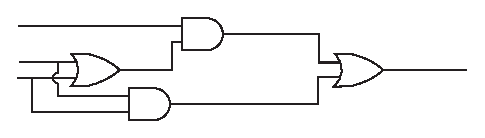
\includegraphics{slika02_log1}}

 \put(1,15.5){$a$}
 \put(1,9.5){$b$}
 \put(1,6.57){$c$}

{\scriptsize
 \put(24,9.5){$b \vee c$}
 \put(41,4.25){$b\wedge c$}
 \put(42, 16){$a\wedge (b\vee c)$}

 \put(68.5, 10){$G(a, b, c)$}
 }

\end{picture}}\end{center}
\end{solution}

\begin{example}
Nacrtajmo logi\v{c}ki element za implikaciju.
\end{example}
\begin{solution}
Poznato nam je da vrijedi $a\Rightarrow b=\overline{a}\vee b$.
Na sljede\'{c}oj slici je pripadni logi\v{c}ki sklop.
%\begin{center}
%\includegraphics[width=6cm]{zad64str31.eps}
%\FIXME{slika0211}
%\end{center}
\begin{center}
%\fbox
{
\small
\setlength\unitlength{1mm}
\begin{picture}(50,10)
 \put(3,0){\includegraphics{slika02_log2}}

 \put(0,6){$a$}
 \put(0,1){$b$}
 \put(20, 8){$\overline{a}$}
 \put(41, 4){$\overline{a}\vee b$}
\end{picture}
}
\end{center}
\end{solution}




\begin{example}
Nacrtajmo logi\v{c}ki element za funkciju algebre sudova
$$\ F(x,y,z)=(x\vee z)\Rightarrow (y\wedge
\overline{z}).$$
\end{example}

\begin{solution} Semanti\v{c}ka tablica za ovu funkciju je
\begin{center}
\begin{tabular}{c|c|c|c|c|c|c|c}
$x$ & $y$ & $z$ & $\overline{z}$ & $y\wedge \overline{z}$ & $x\vee z$ & $(x\vee
z)\Rightarrow (y\wedge \overline{z})$ & bazi\v{c}ne konjunkcije \\ \hline
1 & 1 & 1 & 0 & 0 & 1 & 0 &  \\
1 & 1 & 0 & 1 & 1 & 1 & 1 &   $x\wedge y\wedge \overline{z}$ \\
1 & 0 & 1 & 0 & 0 & 1 & 0 &  \\
1 & 0 & 0 & 1 & 0 & 1 & 0 &  \\
0 & 1 & 1 & 0 & 0 & 1 & 0 &  \\
0 & 1 & 0 & 1 & 1 & 0 & 1 &   $\overline{x}\wedge y\wedge \overline{z}$ \\
0 & 0 & 1 & 0 & 0 & 1 & 0 &  \\
0 & 0 & 0 & 1 & 0 & 0 & 1 &   $\overline{x}\wedge \overline{y}\wedge \overline{z} $\\
\end{tabular}%
\end{center}

$DNF(F)=(x\wedge
y\wedge
\overline{z})\vee (\overline{x}\wedge y\wedge \overline{z})\vee (\overline{x}%
\wedge \overline{y}\wedge \overline{z})$. Minimizacija ove formule
je formula $F_{m}=\overline{z}\wedge (\overline{x}\vee y).~$Na
slijede\'{c}oj slici prikazan je logi\v{c}ki element za zadanu
funkciju
%\begin{center}
%\includegraphics[width=10cm]{zad65str32.eps}
%\FIXME{slika0212}
%\end{center}
\begin{center}
{
\small
\setlength\unitlength{1mm}
\begin{picture}(82,19)
 \put(3,0){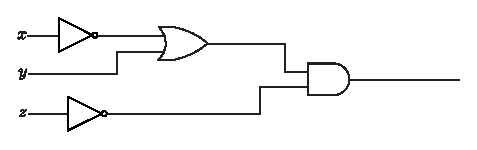
\includegraphics{slika02_log3}}

 \put(20,17.28){$\overline{x}$}
 \put(31,4.5){$\overline{z}$}
 \put(38,16.25){$\overline{x}\vee y$}
 \put(60, 10.2){$F(x,y,z)$}
\end{picture}
}
\end{center}
\end{solution}

\section{Predikati}

Predikate je u matematiku uveo jedan od utemeljitelja
matema\v{c}ke logike Gottlob Frege, godine 1880.

Sudovi nisu dovoljni za izricanje svih tipova tvrdnji u
matematici.
Osim njih u matematici se koriste i drugi tipovi re\v{c}enica. U tim re\v{c}%
enicama iznose se tvrdnje u kojima se jedan ili vi\v{s}e elemenata
nekog skupa povezuju s nekim svojstvom. Glavno svojstvo strukture
takvih re\v{c}enica je to da one sadr\v{z}e subjekt (element(e)
nekog skupa) i predikat (svojstvo koje se pridru\v{z}uje navedenom
elementu(ima)). Zbog toga se takve re\v{c}enice zovu predikati.



\begin{example}
Koje su od sljede\'{c}ih izjava sudovi?
\begin{enumerate}
\item ``V. Jagi\'{c} \v{z}ivio je u Vara\v{z}dinu''
\item ``Osoba  $x$ \v{z}ivi u Vara\v{z}dinu''
\item ``$5$ je prim broj''
\item ``$x$ je prim broj''
\item ``Kuko\v{c} je vi\v{s}i od Jordana''
\item  ``$x$ je ve\'{c}e od $y$''
\end{enumerate}
\end{example}

\begin{solution}
 Re\v{c}enice 1, 3 i 5 su sudovi. Oni koji poznaju hrvatsku knji\v{z}evnost
 znaju i to da je prva re\v{c}enica istinit sud, a oni koji znaju ne%
\v{s}to o ko\v{s}arci znaju da je peta re\v{c}enica istinit sud. \v{C}%
injenica da je tre\'{c}a re\v{c}enica istinit sud spada u op\'{c}u
kulturu. Druga i \v{c}etvrta re\v{c}enica imaju zajedni\v{c}ko
svojstvo da iznose
tvrdnje koje se odnose na nepoznatu veli\v{c}inu  $x$ i te re\v{c}enice
postaju sudovi ukoliko se odrede te nepoznate veli\v{c}ine.
Posljednja
re\v{c}enica sadr\v{z}i \v{c}ak dvije takve veli\v{c}ine. Takve re\v{c}enice,
koje sadr\v{z}e tvrdnje o nepoznatim veli\v{c}inama, i koje
postaju sudovi kada se odrede (specificiraju) te nepoznate
veli\v{c}ine, zovu se \textbf{predikati}\index{predikat}. Pri tom se jo\v{s} ka\v{z}e da je
npr. druga re\v{c}enica predikat s jednom varijablom, a posljednja
re\v{c}enica je predikat s dvije
varijable. Za onu vrijednost od $x$ uvr\v{s}tavanjem koje predikat  $P(x)$%
 postaje istinit sud ka\v{z}emo da zadovoljava predikat. Ukoliko uvr\v{s}tavanjem
 neke vrijednosti za $x$ u predikat dobijemo la\v{z}an sud, ka\v{z}e se da ga ta
 vrijednost ne zadovoljava. Tako npr. $5$
zadovoljava predikat  $Prim(x)$:=``$x$~je~prim~broj'',  a
brojevi $1$ i $4$ ga ne
zadovoljavaju. Sli\v{c}no tome predikat $~>(x,y)$: ``$x$ je ve\'{c}e od $y$''
zadovoljava par $(5,4)$ a ne zadovoljava ga par $(4,5)$.
\end{solution}

 Kod rada s predikatima slu\v{z}imo se oznakama koje
mo\v{z}emo sami uvesti, npr.

 Vara\v{z}din($x$):= ``$x$ je \v{z}ivio u Vara\v{z}dinu'',
pa je V(V. Jagi\'{c}):= ``V. Jagi\'{c} je \v{z}ivio u
Vara\v{z}dinu''. Nadalje, stavimo li $K(x,y)$=: ``$x$ je vi\v{s}i
od $y$'', tada je

K(Kuko\v{c}, Jordan):= ``Kuko\v{c} je vi\v{s}i od
Jordana''.

\textrm{U razli\v{c}itim podru\v{c}jima matematike koriste se
standardne oznake za neke predikate koji se \v{c}e\v{s}\'{c}e
javljaju. Takve oznake su npr. }$\leq ,\geq ,=,<,>$\textrm{~dok se
u geometriji koriste }$\parallel
,\perp ,\cong .~$\textrm{Poznavanje ovih oznaka omogu\'{c}uje nam da \v{s}%
estu re\v{c}enicu iz prethodnog primjera jednostavnije zapi\v{s}emo kao }$%
x>y.$

\begin{exercise}
Na koje se geometrijske pojmove odnose predikati
$\parallel ,\perp ,\cong$? Nacrtajte skice na kojima se
pojmovi a i b odnose tako da predikati  $\parallel\!(a,b)$,
$\perp\!(a,b)$ i $\cong\!(a,b)$ postanu istiniti sudovi.
\end{exercise}

\textrm{Informati\v{c}aru je od posebnog interesa
%za informati\v{c}ara
kako
ispitati da li elementi nekog skupa imaju %neko
 odre\dj{}eno
svojstvo (npr. tko je sve od studenata odre\dj{}enog godi\v{s}ta
polo\v{z}io ispit iz matematike?). Taj je problem povezan sa
zapisivanjem predikata. Skup elemenata na koje se odnosi zadani
predikat }$P$\textrm{\ zove se \textbf{univerzum razmatranja}\index{univerzum razmatranja} }$U$\textrm{.
Taj skup za neke predikate nije potrebno posebno odrediti i pri
tom se podrazumijeva da se radi o najop\'{c}enitijem skupu na koji
se promatrani predikat mo\v{z}e primjeniti. Ukoliko pak se
promatrano svojstvo koje se opisuje predikatom ispituje na odre\dj
enom podskupu nekog ve\'{c}eg skupa potrebno ga je odrediti. Npr.,
ukoliko se govori o
predikatu }$Prim(x)~$\textrm{onda se podrazumijeva da ima smisla prou\v{c}%
avati istinitost sudova koji se formiraju tako da se za x uzimaju
prirodni brojevi. Ukoliko se u prou\v{c}avanju ovog svojstva
ograni\v{c}imo na prirodne brojeve manje od }$10$\textrm{, onda je
potrebno naglasiti da je univerzum razmatranja }$U=\left\{ x\mid
x\in \mathbb{N}\wedge x<10\right\}$. Predikat se
zapisuje pomo\'{c}u tablice u kojoj se elementima iz
univerzuma razmatranja pridru\v{z}uje istinitost suda koji se dobije uvr\v{s}%
tavanjem vrijednosti varijable u predikat. Za tablicu predikata
\v{c}esto se koristi i pojam \textbf{matrica predikata}\index{matrica predikata}.

\begin{example}
Napi\v{s}imo tablicu predikata za predikat
$Prim(x):=$``x je prim broj'' ako je univerzum razmatranja
$U=\left\{ x\mid x\in \mathbb{N}\wedge x<10\right\}$.
\end{example}
\begin{solution}
Tablica predikata:
\begin{center}
\begin{tabular}{l|l|l|l|l|l|l|l|l|l}
$x$ & 1 & \textrm{2} & \textrm{3} & \textrm{4} &
\textrm{5}
& \textrm{6} & \textrm{7} & \textrm{8} & \textrm{9} \\ \hline
$v(P(x))$ & 0 & 1 & 1 &
0 &
1 & 0 & 1 & 0 & 0%
\end{tabular}
\end{center}
%\end{center}
\end{solution}


\begin{example}
Zapi\v{s}imo predikat $>(x,y):=\text{``}x>y\text{''}$ ako je
univerzum razmatranja $U=\left\{ (x,y)\mid x,y\in
\mathbb{N}\wedge x,y<8\right\} $
\end{example}

\begin{solution}
Ovdje se radi o predikatu s dvije varijable pa trebamo
druga\v{c}iju tablicu.
\begin{center}
\begin{tabular}{r|lllllll}
$v(x>y)$ & ${1}$ & ${2}$ & ${3}$ &
$4$
& ${5}$ & ${6}$ & ${7}$ \\
\hline
${1}$ & ${0}$ & ${0}$ & ${0}$ & ${0}$ & $%
{0}$ & ${0}$ & ${0}$ \\
${2}$ & ${1}$ & ${0}$ & ${0}$ & ${0}$ & $%
{0}$ & ${0}$ & ${0}$ \\
${3}$ & ${1}$ & ${1}$ & ${0}$ & ${0}$ & $%
{0}$ & ${0}$ & ${0}$ \\
${4}$ & ${1}$ & ${1}$ & ${1}$ & ${0}$ & $%
{0}$ & ${0}$ & ${0}$ \\
${5}$ & ${1}$ & ${1}$ & ${1}$ & ${1}$ & $%
{0}$ & ${0}$ & ${0}$ \\
${6}$ & ${1}$ & ${1}$ & ${1}$ & ${1}$ & $%
{1}$ & ${0}$ & ${0}$ \\
${7}$ & ${1}$ & ${1}$ & ${1}$ & ${1}$ & $%
{1}$ & ${1}$ & ${0}$%
\end{tabular}
\end{center}
\nopagebreak
\end{solution}

 Neka je $P(x_{1},x_{2},...,x_{n})$ predikat s $n$
varijabli. S obzirom na to koje mogu\'{c}nosti
zadovoljavanja ovog predikata postoje koristi se sljede\'{c}a
terminologija:

\begin{itemize}
\item \textrm{Ako je
}$P(x_{1},x_{2},...,x_{n})~$\textrm{zadovoljen za svaki izbor
}$n$-torke argumenata iz univerzuma razmatranja
$U$, ka\v{z}e se da taj predikat vrijedi u $U$.

\item \textrm{Ako je }$P(x_{1},x_{2},...,x_{n})~$\textrm{zadovoljen za neku }%
$n$\textrm{-torku argumenata iz univerzuma razmatranja }$U$\textrm{, ka\v{z}%
e se da je taj predikat zadovoljiv u }$U~$

\item \textrm{Ako ne postoji }$n$\textrm{-torka argumenata iz
univerzuma
razmatranja }$U$ koja zadovoljava $P(x_{1},x_{2},...,x_{n}),~$
ka\v{z}e se da taj predikat nije zadovoljiv u~$U$.
\end{itemize}

\paragraph{\textrm{Ograni\v{c}avanje varijabli u predikatu.}}
\textrm{Da bi se od predikata dobio sud nu\v{z}no je odrediti ili ograni\v{c}%
iti vrijednost(i) varijable(i) koje sadr\v{z}i predikat. To se
mo\v{z}e napraviti na dva osnovna na\v{c}ina:}

\begin{enumerate}
\item pridru\v{z}ivanjem odre\dj ene vrijednosti varijablama,
\item upotrebom kvantifikatora.
\end{enumerate}
Prvi na\v{c}in smo upoznali tokom dosada\v{s}njeg
obja\v{s}njavanja pojma predikata.


\subsection{Kvantifikatori}

\subsubsection{Univerzalni kvantifikator}

U matematici se \v{c}esto koriste re\v{c}enice tipa ``Za svaki $x$
vrijedi tvrdnja $P(x)$'' pri \v{c}emu je $P(x)$
zadani predikat. Ova fraza kra\'{c}e se pi\v{s}e  ``$\forall xP(x)$''.
Znak  $\forall$  zove se univerzalni kvantifikator, a
ovisno o konstrukciji re\v{c}enice on\ se \v{c}ita ``za svaki'',
``za sve'', ``za proizvoljan'' i sl. Budu\'{c}i da je upotrebom ovog
znaka odre\dj{}eno na koje vrijednosti od  $x$ se odnosi
tvrdnja iz predikata $P(x)$, re\v{c}enica $\forall
xP(x)$ je sud za koji vrijedi:

\begin{definition}
Sud $\forall x\ P(x)$ je istinit onda i samo onda ako $P(x)$
vrijedi u  $U$.
\end{definition}

\begin{exercise}
\rjesenje{1.~$\top$, 2.~$\bot$, istinit u $\mathcal{U}=\{5\}$, 3.~$\bot$, istinit u $\mathcal{U}=\{1\}$}
Odredite istinitost sljede\'{c}ih sudova za
$U=\mathbb{Z}$. Za sudove koji nisu istiniti u tom univerzumu
razmatranja, odredite najmanji univerzum razmatranja u kojem su
istiniti.
\begin{exerciseslots}
\hspace{1cm}
\= \exnumslot{${\forall x}\left[ x<x+1\right] $}
\= \exnumslot{${\forall x}\left[ x=5\right] $}
\\
\> \exnumslot{${\forall x\forall y}\left[ x+y>x\right] $}
%\> \exnumslot{}
%\\
%\> \exnumslot{}
%\> \exnumslot{}
%\\
%\> \exnumslot{}
%\> \exnumslot{}
\end{exerciseslots}
\end{exercise}

\subsubsection{Egzistencijalni kvantifikator}
Re\v{c}enice tipa ``Za neki $x$ vrijedi tvrdnja $P(x)$'', tj. re\v{c}enice koje
 su logi\v{c}ki ekvivalentne s re\v{c}enicom ``postoji takav $x$ da je  $P(x)$ istinit
sud'' mogu se kra\'{c}e zapisati kao ``$\exists xP(x)$''. Znak $\exists$
zove se egzistencijalni kvantifikator i \v{c}ita se ``za
neki'', ``postoji takav'', ``za najmanje jedan''.

\begin{definition}
Sud $\exists xP(x)$ je istinit onda i samo onda ako je $P(x)$
zadovoljiv u $U$.
\end{definition}

Postoji i varijacija ovog kvantifikatora kojom se
izra\v{z}ava tvrdnja da $P(x)$ vrijedi samo za jednu vrijednost od $x$.
Oznaka za taj kvantifikator je $\exists !$, a fraza $\exists !x$
\v{c}ita se ``postoji $1$ i samo $1$ $x$'',
 ``postoji jedinstven $x$'' i sl.

\begin{exercise}
\rjesenje{1.~$\top$, 2.~$\bot$, 3.~$\bot$, 4.~$\top$, 5.~$\bot$, istinit u npr.~$\mathcal{U}=\{1\}$}
Odredite istinitost sljede\'{c}ih sudova za $U=\Z$. Za sudove
koji nisu istiniti u tom univerzumu razmatranja, odredite najmanji
univerzum razmatranja u kojem su istiniti.
\begin{exerciseslots}
\hspace{1cm}
\= \exnumslot{${\exists x}\left[ x<x+1\right] $}
\= \exnumslot{${\exists x}\left[ x=5\right] $}
\\
\> \exnumslot{${\exists x}\left[ x=x+1\right] $}
\> \exnumslot{${\exists !x}\left[ x=5\right] $}
\\
\> \exnumslot{${\exists !x}\left[ x=x\cdot x\right] $}
%\> \exnumslot{}
%\\
%\> \exnumslot{}
%\> \exnumslot{}
\end{exerciseslots}
%\begin{enumerate}
%\item
%
%\item
%
%\item
%
%\item
%
%\item
%\end{enumerate}
\end{exercise}

\subsection*{Veza izme\dj{}u kvantifikatora i logi\v{c}kih operacija}

Da bi se u odre\dj{}enom univerzumu razmatranja ispitala
istinitost sudova $\forall xP(x)$, $\exists xP(x)$ i $\exists
!xP(x)$ potrebno je ove sudove zapisati u obliku na koji
je mogu\'{c}e primjeniti poznati postupak ispitivanja istinitosti
slo\v{z}enih sudova s obzirom na istinitosne vrijednosti sudova od
kojih su sastavljeni. Ako je zadan
predikat $P\left( x\right)$ i pripadni univerzum\ razmatranja $U(x)$,
tada su sljede\'{c}i sudovi ekvivalentni:
\begin{eqnarray*}
\forall xP(x) &\iff &(P(x_{1})\wedge P(x_{2})\wedge
...\wedge
P(x_{n})) \\
\exists xP(x) &\iff &(P(x_{1})\vee P(x_{2})\vee
...\vee
P(x_{n})) \\
\exists !xP(x) &\iff &((P(x_{1})\wedge \neg
P(x_{2})\wedge ...\wedge \neg P(x_{n}))\vee \\
& &
\qquad \vee(\neg
P(x_{1})\wedge P(x_{2})\wedge ...\wedge \neg P(x_{n}))\vee\\
& & \qquad \qquad \vee
(\neg P(x_{1})\wedge \neg P(x_{2})\wedge ...\wedge P(x_{n})))
\end{eqnarray*}


\subsection*{Negacija, predikat i kvantifikator}

\begin{example}
Sljede\'{c}e sudove-re\v{c}enice
\begin{exerciseslots}
\hspace{1cm}
\= \exslot{``$P$ je istinit za svaki $x$'' }
\= \exslot{``$P$ je istinit za neki $x$''}
\\
\> \exslot{``$P$ je la\v{z}an za svaki  $x$''}
\> \exslot{``$P$ je la\v{z}an za neki  $x$''}
\end{exerciseslots}
pridru\v{z}imo
simboli\v{c}kim zapisima:
\begin{exerciseslots}
\hspace{1cm}
\= \exnumslot{${\forall xP}\left( x\right) $ }
\= \exnumslot{${\exists xP}\left( x\right) $}
\\
\> \exnumslot{${\forall x\neg P}\left( x\right) $}
\> \exnumslot{${\exists x\neg P}\left( x\right) $}
\\
\> \exnumslot{${\neg }\left( \forall xP\left( x\right) \right) $}
\> \exnumslot{${\neg }\left( \exists xP\left( x\right) \right) $}
\\
\> \exnumslot{${\neg }\left( \forall x\neg P\left( x\right)
\right) $ }
\> \exnumslot{${\neg }\left( \exists x\neg P\left( x\right)
\right) {.}$}
\end{exerciseslots}
%\begin{enumerate}
%
%\item ${\forall xP}\left( x\right) $
%
%\item ${\exists xP}\left( x\right) $
%
%\item ${\forall x\neg P}\left( x\right) $
%
%\item ${\exists x\neg P}\left( x\right) $
%
%\item ${\neg }\left( \forall xP\left( x\right) \right) $
%
%\item ${\neg }\left( \exists xP\left( x\right) \right) $
%
%\item ${\neg }\left( \forall x\neg P\left( x\right)
%\right) $
%
%\item ${\neg }\left( \exists x\neg P\left( x\right)
%\right) {.}$
%\end{enumerate}
\end{example}
\begin{solution}
1.~a, 2.~b, 3.~c, 4.~d, 5.~d, 6.~c, 7.~b, 8.~a
\end{solution}



Ukoliko tvrdnja sadr\v{z}i predikat, negaciju i kvantifikator vrijede sljede%
\'{c}e ekvivalencije
\begin{eqnarray*}
\neg \forall xP(x) &\iff &\exists x\neg P(x) \\
\neg \exists xP(x) &\iff &\forall x\neg P(x)
\end{eqnarray*}
Ponekad se \v{c}uju re\v{c}enice koje zbunjuju zbog kombinacija
negacije i kvantifikatora koje se javljaju u njima.

\begin{example}
Re\v{c}enicu ``Nije istina da neki misle da general nije kriv''
zapi\v{s}ite pomo\'{c}u predikata $K(x)$:``$x$ misli da je general
kriv'', negacije i kvantifikatora. Zatim na temelju svojstava
odnosa negacije i kvantifikatora zamijenite tu re\v{c}enicu
jednostavnijom.
\end{example}

``Nije istina da neki misle da general nije kriv'' $\leftrightarrow
\neg (\exists x\neg K(x))\Leftrightarrow \neg
(\neg \forall xK(x))\Leftrightarrow \forall
xK(x)\leftrightarrow $ ``Svi misle da je general kriv''

\begin{exercise}
\rjesenje{1.~$\forall x\exists y (x<y)$ $\mathcal{U}=\R$,
2.~$\forall x\exists y (y=\sqrt{x})$ $\mathcal{U}=\R^{+}$,
3.~$\forall x\forall y \exists z   (x+y=z)$ $\mathcal{U}=\R$,
4.~$\forall x\exists y (y>x)$ $\mathcal{U}=\R$,
5.~$\exists \forall y (x>y) \mathcal{U}=\R$.
}
 Zapi\v{s}ite sljede\'{c}e re\v{c}enice pomo\'{c}u
kvantifikatora i predikata, te odredite njihovu istinitost.

\begin{enumerate}
\item  Ne postoji najve\'{c}i realan broj.

\item  Svi pozitivni realni brojevi imaju realni drugi
korijen.

\item  Postoji jedinstvena suma svaka dva realna broja.

\item  Za svaki realan broj postoji neki drugi realan broj
koji je od prvog ve\'{c}i.

\item  Postoji realan broj koji je ve\'{c}i od svakog
drugog realnog broja.
\end{enumerate}
\end{exercise}



Zbog svojstava odnosa izme\dj{}u kvantifikatora i logi\v{c}kih
operacija tvrdnje koje sadr\v{z}e predikate, kvantifikatore i
logi\v{c}ke operacije mogu se zapisati u razli\v{c}itim
logi\v{c}ki ekvivalentnim oblicima. Osim ekvivalencija koje se
odnose na negaciju i kvantifikatore, koje smo ve\'{c} pokazali,
vrijede i sljede\'{c}e relacije (nisu sve ekvivalencije):
\begin{eqnarray*} (\forall xP(x)\wedge \forall xQ(x))
&\Leftrightarrow &\forall x(P(x)\wedge
Q(x)) \\
(\forall xP(x)\vee \forall xQ(x)) &\Rightarrow &\forall x(P(x)\vee Q(x)) \\
\exists x(P(x)\wedge Q(x)) &\Rightarrow &(\exists xP(x)\wedge
\exists xQ(x))
\\
(\exists xP(x)\vee \exists xQ(x)) &\Leftrightarrow &\exists
x(P(x)\vee Q(x))
\protect\end{eqnarray*}%


\subsection*{Sudovi s vi\v{s}e kvantifikatora}

\textrm{Ukoliko je zadan predikat s vi\v{s}e varijabli, mogu\'{c}e
je istovremeno vi\v{s}e njih ograni\v{c}iti kvantifikatorima i
dobiti sud. Pri tom treba paziti na to kojim se redoslijedom
pi\v{s}u kvantifikatori jer to utje\v{c}e na smisao re\v{c}enice
kojom se izri\v{c}e sud, odnosno na njegovu logi\v{c}ku
vrijednost. Bez detaljnijeg prou\v{c}avanja zakonitosti veza
izme\dj u razli\v{c}itih kombinacija kvantifikatora i smisla
sudova u kojima se te kombinacije koriste, na sljede\'{c}im
primjerima se pokazuje da zamjene redoslijeda pisanja
kvantifikatora i varijabli bitno mijenjaju smisao i istinitost
suda u kojem se javljaju.}

\begin{exercise}
\rjesenje{a)~svaka je osoba u braku s nekim, b)~postoji osoba koja je sa svima u braku}
Neka je $P(x,y)$:=``Osoba $x$ u braku je s osobom $y$''. Neka je  $U$
  neprazan skup bra\v{c}nih parova.  Izrazite rije\v{c}ima sudove
 a)~$\forall x\exists yP\left( x,y\right) $  i  b)~$\exists
y\forall xP\left( x,y\right)$, te odredite njihovu
istinitost.
\end{exercise}

\begin{exercise}
\rjesenje{
1.~$\top$,
2.~$\bot$,
3.~$\top$,
4.~$\top$,
5.~$\top$,
6.~$\bot$}
{Neka je }$U =\mathbb{Z}$. Odredite istinitost
sljede\'{c}ih sudova
\begin{exerciseslots}
\hspace{1cm}
\= \exslot{${\forall x\exists y}\left[ x+y=0\right] $}
\= \exslot{${\exists y\forall x}\left[ x+y=0\right] $}
\\[0.35ex]
\> \exslot{${\forall x\forall y\exists !z}\left[ x+y=z\right] $}
\> \exslot{${\exists !x}\left[ x\cdot 6=0\right] $}
\\[0.35ex]
\> \exslot{${\exists !x\forall y}\left[ x\cdot y=0\right] $}
\> \exslot{${\forall y\exists !x}\left[ x\cdot y=0\right] $}
%\\
%\> \exslot{}
%\> \exslot{}
\end{exerciseslots}
%
%\begin{enumerate}
%\item ${\forall x\exists y}\left[ x+y=0\right] $
%
%\item ${\exists y\forall x}\left[ x+y=0\right] $
%
%\item ${\forall x\forall y\exists !z}\left[ x+y=z\right] $
%
%\item ${\exists !x}\left[ x\cdot 6=0\right] $
%
%\item ${\exists !x\forall y}\left[ x\cdot y=0\right] $
%
%\item ${\forall y\exists !x}\left[ x\cdot y=0\right] $
%\end{enumerate}
\end{exercise}

Dopu\v{s}tene su sljede\'{c}e zamjene kombinacija
kvantifikatora:
\begin{eqnarray*}
\forall x\forall y &\Leftrightarrow &\forall y\forall x \\
\exists x\exists y &\Leftrightarrow &\exists y\exists x
\end{eqnarray*}


\bigskip

\section{Dodatak}

\projekti
\begin{project}
  Augustus De Morgan
\end{project}

\begin{project}
  Osnovni pojmovi i definicije operacija neizrazite (fuzzy)
logike.
\end{project}


\medskip

%\subsection{Va\v{z}ni pojmovi u poglavlju}
%
%Sud
%
%Operacije
%
%Predikat
%
%
%\bigskip


%\begin{widepar}
%\begin{multicols}{2}[
%\zadacizaponavljanje
%]

\zadacizaponavljanje

\begin{exercise}
Koje od sljede\'{c}ih izjava predstavljaju sudove?

\begin{enumerate}[\quad a)]
\item Darwinizam je trenutno znanstveno prihva\'{c}ena teorija
evolucije (\textquotedblleft natura non facit
saltum\textquotedblright ).

\item Eksponencijalna spirala naj\v{c}e\v{s}\'{c}i je
matemati\v{c}ki oblik u prirodi.

\item Evolucijsko stablo je binarno stablo.


\item \textquotedblleft Blended learning\textquotedblright\ je
kombinacija e-learninga i tradicionalnog podu\v{c}avanja.
\end{enumerate}
\end{exercise}

\begin{exercise}
Napi\v{s}ite tablice istinitosti za sljede\'{c}e sudove
\begin{enumerate}[\quad a)]
\item $x\Rightarrow \lnot \left( y\vee x\right) ,$

\item $\left( x\wedge y\right) \vee \left( \bar{x}\Rightarrow
y\right) $
\end{enumerate}
\end{exercise}


%\end{enumerate}
%
%
%%\bigskip \textbf{Matemati\v{c}ka logika}
%
 \begin{exercise}
  Poka\v{z}ite da su sljede\'{c}e formule semanti\v{c}ki jednake%
\begin{eqnarray*}
F\left( x,y,z\right) &=&\left( \left( x\Rightarrow y\right) \wedge \left(
x\Rightarrow z\right) \right) \\
G\left( x,y,z\right) &=&\left( x\Rightarrow \left( y\wedge z\right) \right) .
\end{eqnarray*}
\end{exercise}

 \begin{exercise}
    Mo\v{z}e li formula s jednom varijablom biti kontradikcija, odnosno
tautologija?
 \end{exercise}

\begin{exercise}  Minimizirajte i nacrtajte logi\v{c}ki elemement funkcije algebre sudova%
\[
F\left( x,y,z\right) =\left( \left( \bar{x}\wedge \bar{z}\right)
\Leftrightarrow \left( y\Rightarrow x\right) \right) \vee \left( z\vee
\left( \bar{z}\wedge \bar{y}\right) \right) .
\]
%\end{enumerate}
%
%%\bigskip \textbf{Predikati}
%
%\begin{enumerate}
\end{exercise}



 \begin{exercise}
     Negirajte sljede\'{c}e re\v{c}enice.

\begin{enumerate}
\item Svi labudovi su bijeli.

\item Ne postoji najve\'{c}i broj.

\item Na\v{s} je gradona\v{c}elnik dobar \v{c}ovjek i lo\v{s} politi\v{c}ar.

\item Ivo govori engleski i francuski.
\end{enumerate}
 \end{exercise}


\begin{exercise}
Napi\v{s}ite obrat po kontrapoziciji sljede\'{c}ih tvrdnji.

\begin{enumerate}
\item Ako \v{z}ivotinja ima rogove tada ona nije ptica.

\item U\v{c}it \'{c}u matematiku ako mi se za to plati.

\item Ako mislim onda postojim.
\end{enumerate}
\end{exercise}



\begin{exercise}
 Koje su od sljede\'{c}ih tvrdnji istinite? Obrazlo\v{z}ite za\v{s}to.
 \begin{exerciseslots}
\hspace{1cm}
\= \exslot{$\forall x\left( x-1\geq x+1\right) \left( x\in \mathbb{R}\right) $}
\= \exslot{$\exists !x\left( x+2=4x+3\right) \left( x\in \mathbb{N}\right) $}
\\
\> \exslot{$\exists x\left( x^{2}+2=2^{x}\right) \left( x\in \mathbb{R}\right) $}
\> \exslot{$\exists x\left( x^{2}=3\right) \left( x\in \mathbb{Q}\right) $}
\\
\> \exslot{$\forall x\exists !y\left( y=x^{2}\right) \left( x\in \mathbb{N}%
\right) $}
%\> \exslot{}
%\\
%\> \exslot{}
%\> \exslot{}
\end{exerciseslots}
\end{exercise}
%\end{enumerate}



%
%  semanticke
%
\begin{exercise}
%\rjesenje{TODO}
Izradite semanti\v{c}ke tablice za formule za deduktivno
zaklju\v{c}ivanje i uvjerite se da su to tautologije.
\end{exercise}

\begin{exercise}
\rjesenje{Nije.}
Provjerite da li je funkcija
$
\left( \neg \left( x\wedge y\right) \Leftrightarrow x\right)
\Rightarrow y
$
tautologija.
\end{exercise}

\begin{exercise}
\rjesenje{Nisu.}
 Ispitajte da li su funkcije $F_{1}=\left( \bar{x}\vee
z\right)
\Rightarrow \left( x\Rightarrow y\right) $ i $F_{2}=\left( \bar{x}%
\vee y\right) \vee \left( y\wedge \bar{z}\right) $ semanti\v{c}ki
jednake (tj. imaju li one jednake vrijednosti za odgovaraju\'{c}e
vrijednosti varijabli). Da li su one sintakti\v{c}ki jednake (tj.
mo\v{z}e li se jedna svesti na drugu)?
\end{exercise}

\begin{exercise}
\rjesenje{$DNF=(x\wedge  y \wedge \bar{z})
\vee (x\wedge \bar{y} \wedge \bar{z})
\vee (\bar{x} \wedge y \wedge \bar{z})
\vee (\bar{x}\wedge \bar{y}\wedge z)
\vee (\bar{x}\wedge \bar{y}\wedge \bar{z})$
$F_{\min} = (y\wedge \bar{z})\vee (\bar{y}\wedge z) \vee (\bar{x}\wedge \bar{z})$
}
 Odredite disjunktivnu normalnu formu funkcije
\begin{equation*}
\left( \left( x\vee y\right) \wedge z\right) \Leftrightarrow \left( \bar{y}%
\wedge x\right) .
\end{equation*}%
 Zatim minimizirajte dobivenu formu i nacrtajte logi\v{c}ki
element.
\end{exercise}


\begin{exercise}
Neka je $U= \{ \text{Ivo}(I)$, $\text{Jo\v{z}a}(J)$, $\text{Ana}(A)$, $\text{Mato}(M)\}$,
a predikat $\text{Otac}(x,y):=$``$y$ je otac od $x$''.
Znaju\'{c}i da je ovaj predikat zadovoljen samo za parove
$(I,J)$, $(A,J)$ i $(J,M)$ odredite istinitost sljede\'{c}ih sudova:
\rjesenje{
1.~$\top$,
2.~$\bot$,
3.~$\bot$,
4.~$\top$,
5.~$\bot$,
6.~$\bot$,
7.~$\bot$.
}
\FIXME{Otac mathop}
\begin{enumerate}
\item ${\exists x\,\text{Otac}(x,J)}$

\item ${\exists !x \text{Otac}(x,J)}$

\item ${\forall x \text{Otac}(x,J)}$

\item ${\exists x\exists y \text{Otac}(x,y)}$

\item ${\exists x\forall y \text{Otac}(x,y)}$

\item ${\forall x\exists y \text{Otac}(x,y)}$

\item ${\exists y\forall x \text{Otac}(x,y)}$
\end{enumerate}
\end{exercise}

\begin{exercise}
Zadan je predikat $P(x,y,z):x-y=z$. Napi\v{s}ite pomo\'{c}u
ovog predikata i kvantifikatora sljede\'{c}e sudove
\rjesenje{
1.~$\forall x\forall
y\exists zP(x,y,z))$
2.~$\forall x \forall y \exists z P(x, z, y)$,
3.~$\exists!x \forall y P(y, x, y)$,
4.~$\forall x P(x, 0, x)$.
}
\begin{enumerate}
\item Za svaki $x$ i $y$ postoji $z$ takav da je $x-y=z$.

\item Za svaki $x$ i $y$ postoji $z$ takav da je $x-z=y$.

\item Postoji jedan i samo jedan $x$ takav da za svaki $y$
 vrijedi $y-x=y$.

\item Kad se $0$ oduzme od bilo kojeg cijelog broja rezultat je
taj cijeli broj.
\end{enumerate}
\end{exercise}

%\end{multicols}
%\end{widepar}

%\cleardoublepage

%\newpage
%\setlength{\columnseprule}{0.01pt}
%\begin{multicols}{4}[\section*{Rje\v{s}enja zadataka}
%\komentar{probni uzorak rje\v{s}enja zadataka}]
%{\scriptsize
%\begin{enumerate}
%\item 15120
%\item DA
%\item NE
%\item
%\item
%\item 15120
%\item DA
%\item NE
%\item
%\item
%\item 15120
%\item DA
%\item NE
%\item
%\item
%\item 15120
%\item DA
%\item NE
%\item
%\item
%\item 15120
%\item DA
%\item NE
%\item
%\item
%\end{enumerate}
%%\printcontents
%%\tableofcontents
%\vfill
%}
%\end{multicols}



%\newpage
%
%
%
%
%
%%\theendnotes
%
%
%\setlength{\columnseprule}{0pt}
%\begin{dokaz}
%dokaz
%\end{dokaz}
%
%\colorbox{myblue!50}{\parbox{\textwidth}{\textcolor{white}{Kreten}}}

	%\input{pogl04_skupovi_relacije}
	%
	%------------------------------------
	%
	%\part{Linearna algebra}
	%
	%
	%\input{pogl05_matrice}
	%\input{pogl07_sustavi_lin_jdbi}
	%
	%
	%------------------------------------
	%
	%\part{Matemati\v{c}ka Analiza}
	%
	%\input{pogl08_realne_fje}
	%\input{pogl09_nizovi}
	%\input{pogl10_limes}
	%\input{pogl11_derivacija}
	%\input{pogl12_primjena_derivacija}
	%\input{pogl13_integrali}
	%------------------------------------



\backmatter



\chapter*{Rje\v{s}enja zadataka}
\addcontentsline{toc}{chapter}{Rje\v{s}enja zadataka}

    \begin{multicols}{2}
    \raggedright
    \makeatletter
    \@starttoc{rjesenja}
    \makeatother
    \end{multicols}

    
\begin{thebibliography}{9}


\addcontentsline{toc}{chapter}{Bibliografija}
{\small
\bibitem{andrews} Andrews G. E., ``\emph{The Geometric Series in Calculus}'', the American Mathematical Monthly, Vol. 105, Number 1, 1998.

\bibitem{barnett} Barnett S., ``\emph{Matrices - Methods and
Applications}'', Oxford applied mathematics and computing science
series, 1900.

\bibitem{chiang} Chiang A.C. , ``\emph{Osnovne metode ekonomije}'', MATE, Zagreb, 1994.
% Chiang, A. C.: Osnovne metode ekonomije, MATE, Zagreb, 1994.


\bibitem{demidovic} Demidovi\v{c} B. P., ``\emph{Zadaci i rije\v{s}eni primjeri iz vi\v{s}e matematike}'', Tehni\v{c}ka knjiga, Zagreb, 1978.

\bibitem{devlin} Devlin K., ``\emph{Sets, Functions and Logic}'',
Chapman \& Hall, 2004.

\bibitem{divjak:erjavec} Divjak B., Erjavec Z., ``\emph{Gospodarska i financijska
matematika}'', TIVA-FOI, Vara\v{z}din 2003.

\bibitem{divjak:hunjak} Divjak B., Hunjak T., ``\emph{Zbirka zadataka iz matematike}'', TIVA-FOI, 2003.

\bibitem{goodaire:parmenter} Goodaire, E. G., Parmenter, ``\emph{Discrete
Mathematics}'', Prentice Hall, Upper Saddle River, 2002.

\bibitem{hughes-hallett} Hughes-Hallett D., Gleason A. M. et al, ``\emph{Calculus}'', J. Wiley \& Sons Inc., 1994.

\bibitem{Hoffmann1} Hoffmann L. D., Bradley G. L., \textit{Finite
mathematics with Calculus}, McGraw-Hill, Inc. 1995.

\bibitem{horvatic} Horvati\'c K., ``\emph{Linearna Algebra I,
II}'', PMF, Zagreb, 1995.

%\bibitem{hortenson} Hortenson


\bibitem{mortensen} Mortensen M. E., ``\emph{Mathematics for Computer Graphics Applications}'', Industrial Press Inc., New York, 1999.

\bibitem{salas} Salas S., Hille E., Etgen G., ``\textit{Calculus: One and several
variables}'', J. Wiley, 1999.

\bibitem{simon} Simon C.P., Blume L., ``\emph{Mathematics for
Economists}'', W.W. Norton\& Co., New York, London 1994.

\bibitem{stanat:mcalister} Stanat D. R., McAllister D. F.,
``\emph{Discrete Mathematics in Computer Science}'', Prentice/Hall
International, 1977.

\bibitem{summers} Summers, J., ``\emph{Test your logic}: Fifty Puzzles in Deductive Reasoning'',
Dover Publications, 1972.

%\bibitem{silas} Silas?,

\bibitem{sikic:novovjekovna} \v{S}iki\'c, Z., ``\emph{Kako je stvarana novovjekovna matematika}'',
�kolska Knjiga, Zagreb, 1989.

\bibitem{taylor:discrete} Ganier R., Taylor J., ``\emph{Discrete Mathematics for New Technology}'', Institute of Physics Publishing, Bristol, 1999.

\bibitem{veljan:starakombinatorika} Veljan, Darko,  ``\emph{Kombinatorika s teorijom grafova}'', \v{S}kolska knjiga, Zagreb, 1989.

\bibitem{vukovic} Vukovi\'c M., ``\emph{Matemati\v{c}ka logika I}'', PMF-MO, Zagreb, 2000.

}


\end{thebibliography}



%   I N D E K S

    \clearpage
    \renewcommand{\indexname}{Kazalo}
    \phantomsection
    \addcontentsline{toc}{chapter}{Kazalo}
    \printindex


\end{document}
